\chapter{Results}
\label{cap:result}

In this chapter, we present the results of various machine learning
approaches used to train the models discussed in \textit{Chapter \ref{cap:contrib}}.
These results are presented using tables and visualizations to
facilitate understanding the benefits and limitations of each decision. The tables and visualizations,
provide a concise and comparative summary of the performance metrics, such as accuracy, AUC and recall. \\

Additionally, we showcase the outcomes of the CAD infrastructure constructed around this thesis.


\section{Metrics}

After training each model and inferring the predictions,
we saved the metrics of interest for each dataset (train, validate, test).
The training information of each training approach is given in \textit{Table \ref{table:trained-models-information}}.
On the other hand, \textit{Table \ref{table:resume-metrics}} provides a summary of the metrics acquired for each model in the different datasets. \\

The accuracy metric in \textit{Table \ref{table:resume-metrics}} represents
the overall performance of the model in the multiclass classification problem with 8 different labels.
However, given the class imbalance, accuracy may not be the most suitable metric to assess the model's performance in this situation.
Instead, metrics like AUC (Area Under the Curve) and recall should be considered,
as they specifically indicate how well the model is performing in classifying melanoma from the other classes. \\

The metrics with a gray background in \textit{Table \ref{table:resume-metrics}}
are from models that incorporated additional regularization techniques, such as dropout or data augmentation.
These models were trained for 40 epochs,
as regularization tends to slow down the minimization of the objective function compared to the other models that were trained for only 20 epochs. \\

\newpage

It is important to mention that the metrics obtained for all models,
both on the validation and test sets, were generated using the Test-Time Augmentation technique.
As explained in previous chapters, this technique functions as an ensemble, contributing to improved performance during inference. \\

Models that used a scheduler during the training stage are denoted with a symbol next to their names.
For reference, the mapping between the scheduler used and the corresponding symbol is provided in \textit{Table \ref{table:scheduler-mapping}}.

\begin{table}[H]
	\centering
	\begin{tabular}{cc}
		\toprule
		\multicolumn{2}{c}{\textbf{Scheduler Mapping}} \\
		\midrule
		$\star$     & Step Learning Rate \\
		$\ast$      & Cosine Annealing Learning Rate \\
	  $\bullet$   & Cosine Annealing Warm Restarts \\
		\bottomrule
	\end{tabular}
  \caption[Scheduler Mapping]
  {\textit{Scheduler Mapping.
  Table by Author}}
	\label{table:scheduler-mapping}
\end{table}

\newpage

\begin{landscape}

\begin{table}
\centering
\begin{tabular}{lccccccccc}
    \toprule
 & Train AUC & Val AUC &  Test AUC & Train Recall & Val Recall &  Test Recall & Train Acc & Val Acc & Test Acc \\
 \midrule
M0 & 0.952 & 0.903 & 0.892 & 0.756 & 0.676 & 0.652 & 0.835 & 0.778 & 0.772 \\
M1 $\star$ & 0.947 & 0.900 & 0.891 & 0.695 & 0.633 & 0.599 & 0.829 & 0.779 & 0.771 \\
M2 $\ast$ & 0.933 & 0.895 & 0.885 & 0.658 & 0.609 & 0.582 & 0.808 & 0.765 & 0.762 \\
M3 $\bullet$ & 0.935 & 0.896 & 0.886 & 0.663 & 0.605 & 0.589 & 0.811 & 0.767 & 0.764 \\
\midrule
\cellcolor{gray!50}M4 & \cellcolor{gray!50}0.886 & \cellcolor{gray!50}0.877 & \cellcolor{gray!50}0.858 & \cellcolor{gray!50}0.478 & \cellcolor{gray!50}0.475 & \cellcolor{gray!50}0.446 & \cellcolor{gray!50}0.757 & \cellcolor{gray!50}0.750 & \cellcolor{gray!50}0.741 \\
\cellcolor{gray!50}M5 $\star$ & \cellcolor{gray!50}0.867 & \cellcolor{gray!50}0.861 & \cellcolor{gray!50}0.842 & \cellcolor{gray!50}0.423 & \cellcolor{gray!50}0.403 & \cellcolor{gray!50}0.395 & \cellcolor{gray!50}0.728 & \cellcolor{gray!50}0.717 &  \cellcolor{gray!50}0.715 \\
\cellcolor{gray!50}M6 $\ast$ & \cellcolor{gray!50}0.874 & \cellcolor{gray!50}0.868 & \cellcolor{gray!50}0.848 & \cellcolor{gray!50}0.451 & \cellcolor{gray!50}0.440 & \cellcolor{gray!50}0.418 & \cellcolor{gray!50}0.738 & \cellcolor{gray!50}0.728 &  \cellcolor{gray!50}0.722 \\
\cellcolor{gray!50}M7 $\bullet$ & \cellcolor{gray!50}0.877 & \cellcolor{gray!50}0.869 & \cellcolor{gray!50}0.849 & \cellcolor{gray!50}0.470 & \cellcolor{gray!50}0.458 & \cellcolor{gray!50}0.432 & \cellcolor{gray!50}0.742 & \cellcolor{gray!50}0.732 &  \cellcolor{gray!50}0.723 \\

\midrule

  Mean &  94.175\% & 89.850\% & 89.850\%  & 69.300\% & 63.075\% & 60.550\% & 82.075\% & 77.225\% & 76.725\% \\
  SD   & 0.921\% & 0.370\% & 0.351\% &  4.509\% & 3.260\% & 3.178\% & 1.327\% & 0.727\% & 0.499\% \\

\midrule

\cellcolor{gray!50}Mean & \cellcolor{gray!50}87.600\% & \cellcolor{gray!50}86.875\% & \cellcolor{gray!50}84.925\% & \cellcolor{gray!50}45.550\% & \cellcolor{gray!50}44.400\% & \cellcolor{gray!50}42.275\% & \cellcolor{gray!50}74.125\% & \cellcolor{gray!50}73.175\% & \cellcolor{gray!50}72.525\% \\
\cellcolor{gray!50}SD & \cellcolor{gray!50}0.787\% & \cellcolor{gray!50}0.655\% & \cellcolor{gray!50}0.660\% & \cellcolor{gray!50}2.445\% & \cellcolor{gray!50}3.084\% & \cellcolor{gray!50}2.175\% & \cellcolor{gray!50}1.204\% & \cellcolor{gray!50}1.372\% &  \cellcolor{gray!50}1.108\% \\

\bottomrule
\end{tabular}
\caption[Model Metrics in Datasets]
  {\textit{Model Metrics in Datasets. Table by Author}}
{\label{table:resume-metrics}}
\end{table}

\end{landscape}


\section{Training}

In this section, we analyze the performance of the models throughout the training process.
Most of the graphics seen in this section were generated using W\&B (Weight \& Biasses).\\


Every pair of models in the set \(S\), \(S=\{\{M0, M4\}, \{M2, M5\}, \{M3, M6\}, \{M4, M8\}\}\),
shares the same scheduler if they were used in the training phase.
However, each pair differs in batch size, the number of epochs, and regularization techniques. \\

We are presenting this comparison to show how regularization affects the training process. Notice that models that suffer of over-fitting were trained by less epochs than models
that implemented regularization techniques.

\subsection{M0 against M4}

\begin{figure}[H]
\centering
    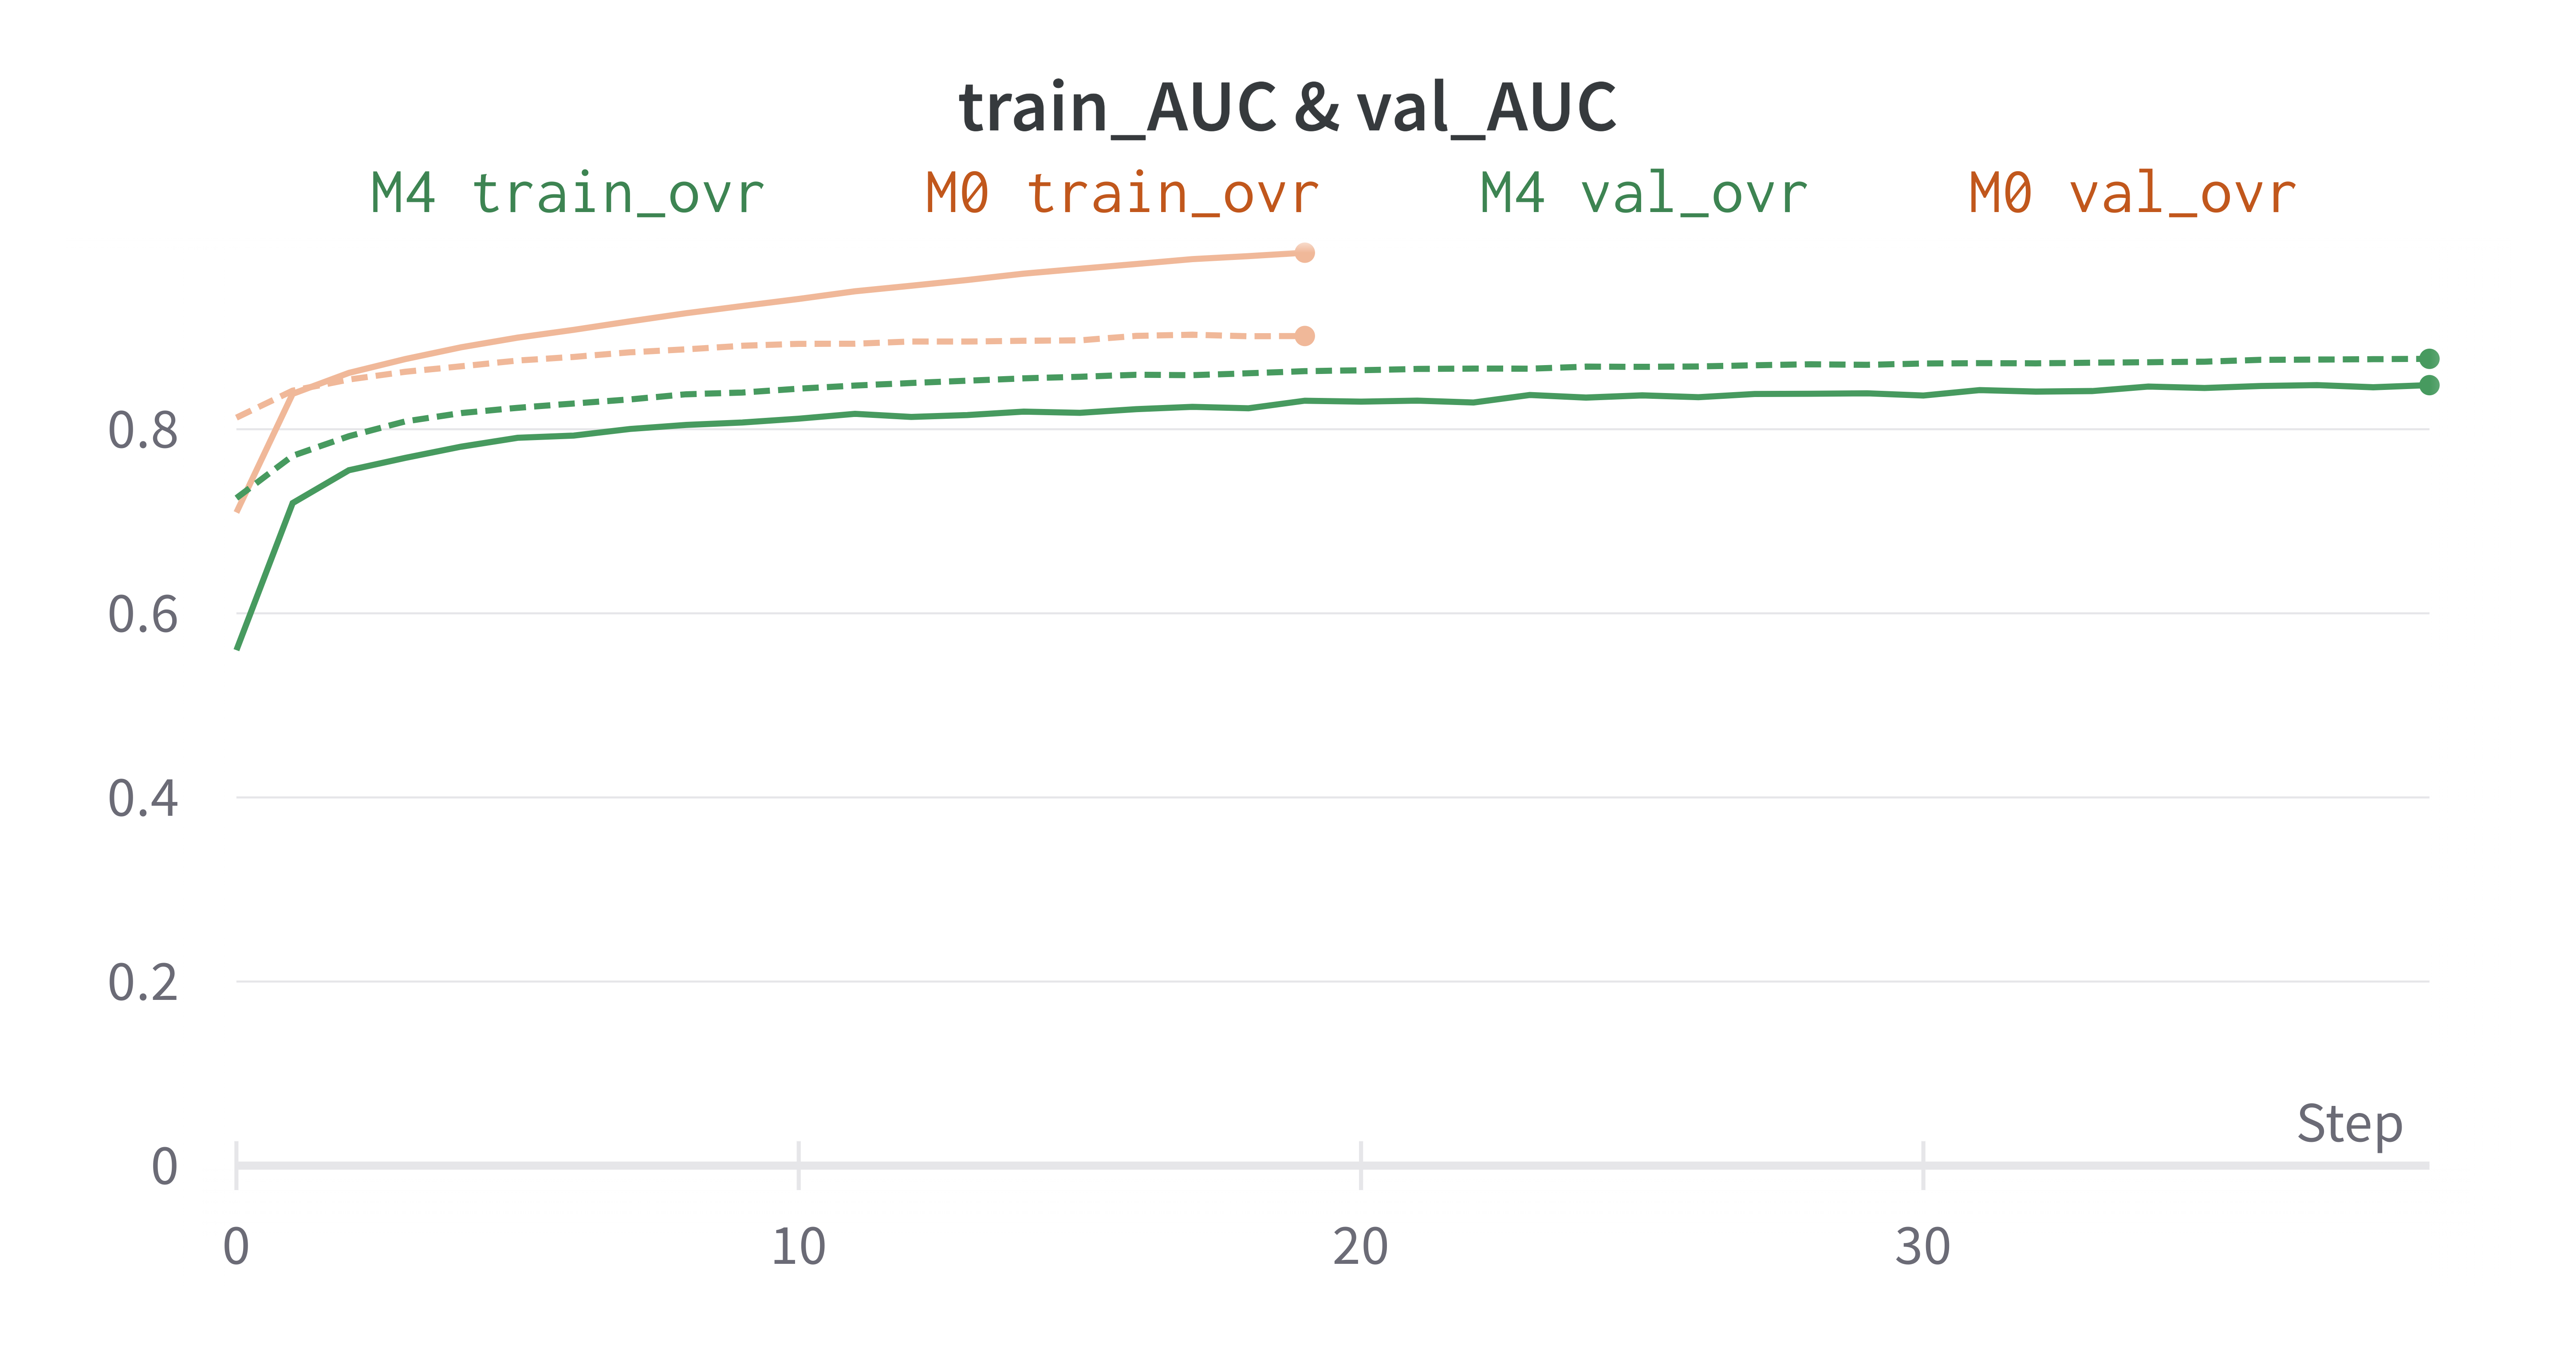
\includegraphics[width=\textwidth]{imatges/results/AUCM0M4.png}
\caption[M0 vs. M4, AUC Train and Validation Curves]{\textit{M0 vs. M4, AUC Train and Validation Curves. Illustration by Author}}
{\label{fig:aucm0m4}}
\end{figure}

\newpage

\begin{figure}[H]
\centering
    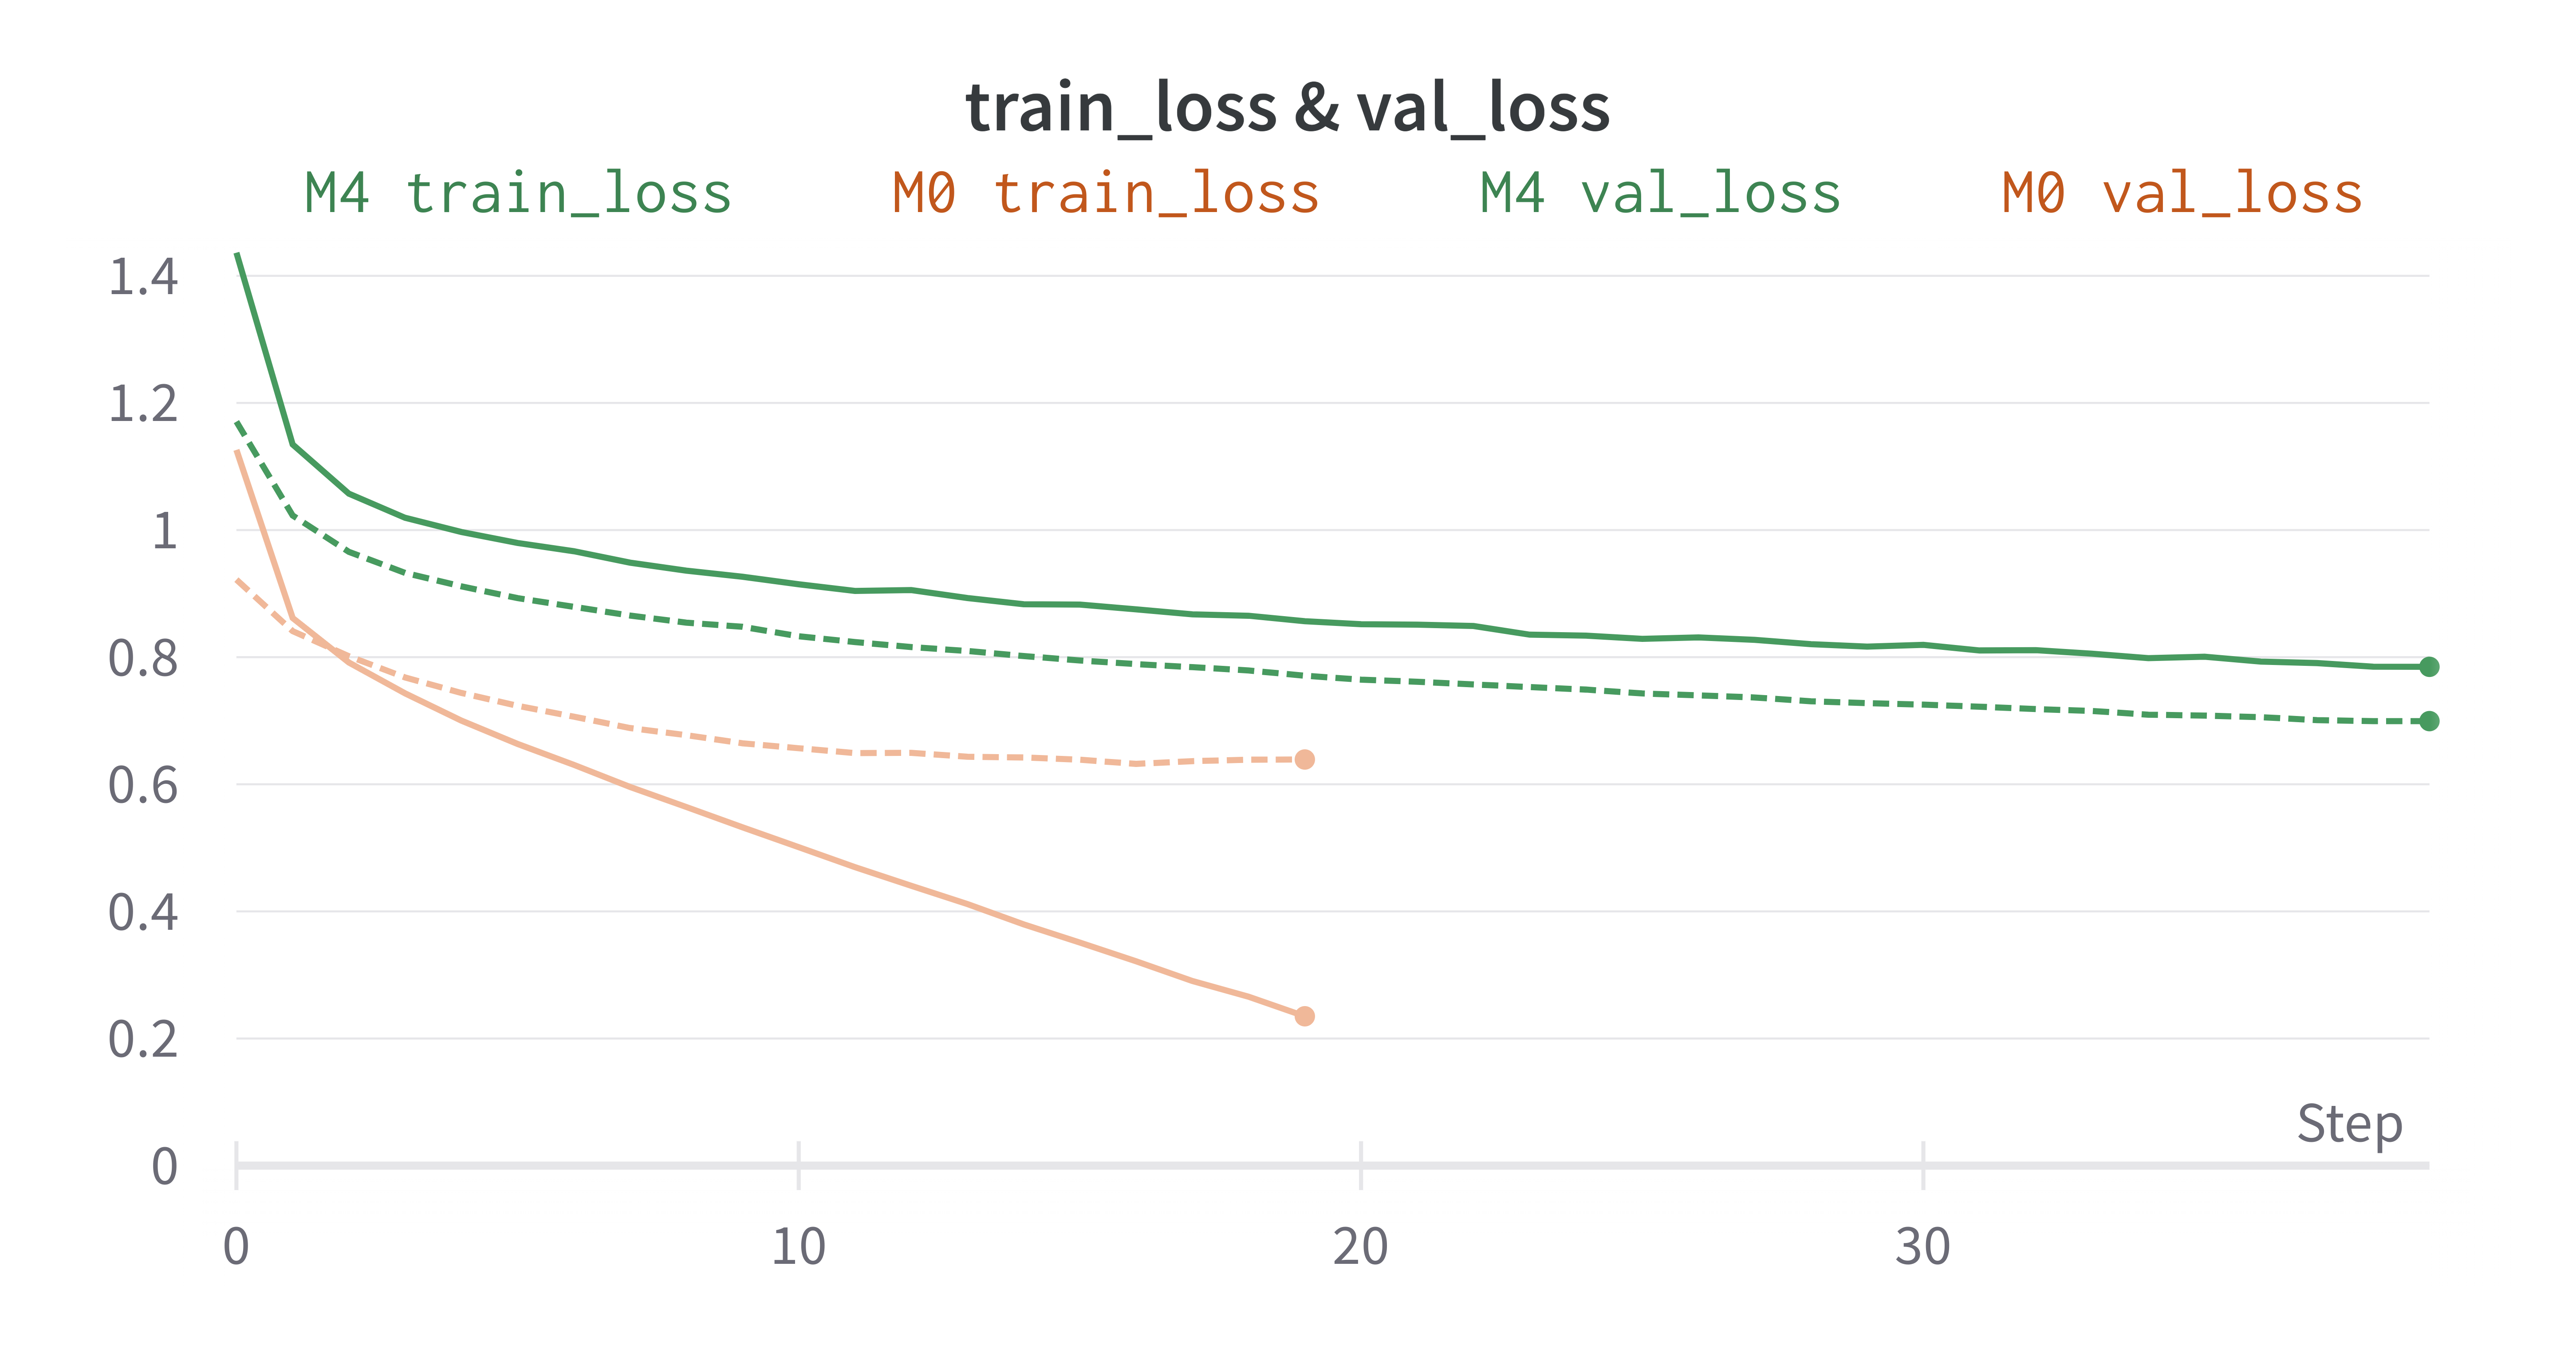
\includegraphics[width=\textwidth]{imatges/results/LossM0M4.png}
\caption[M0 vs. M4, Loss Train and Validation Curves]{\textit{M0 vs. M4, Loss Train and Validation Curves. Illustration by Author}}
{\label{fig:lossm0m4}}
\end{figure}

\begin{figure}[H]
\centering
    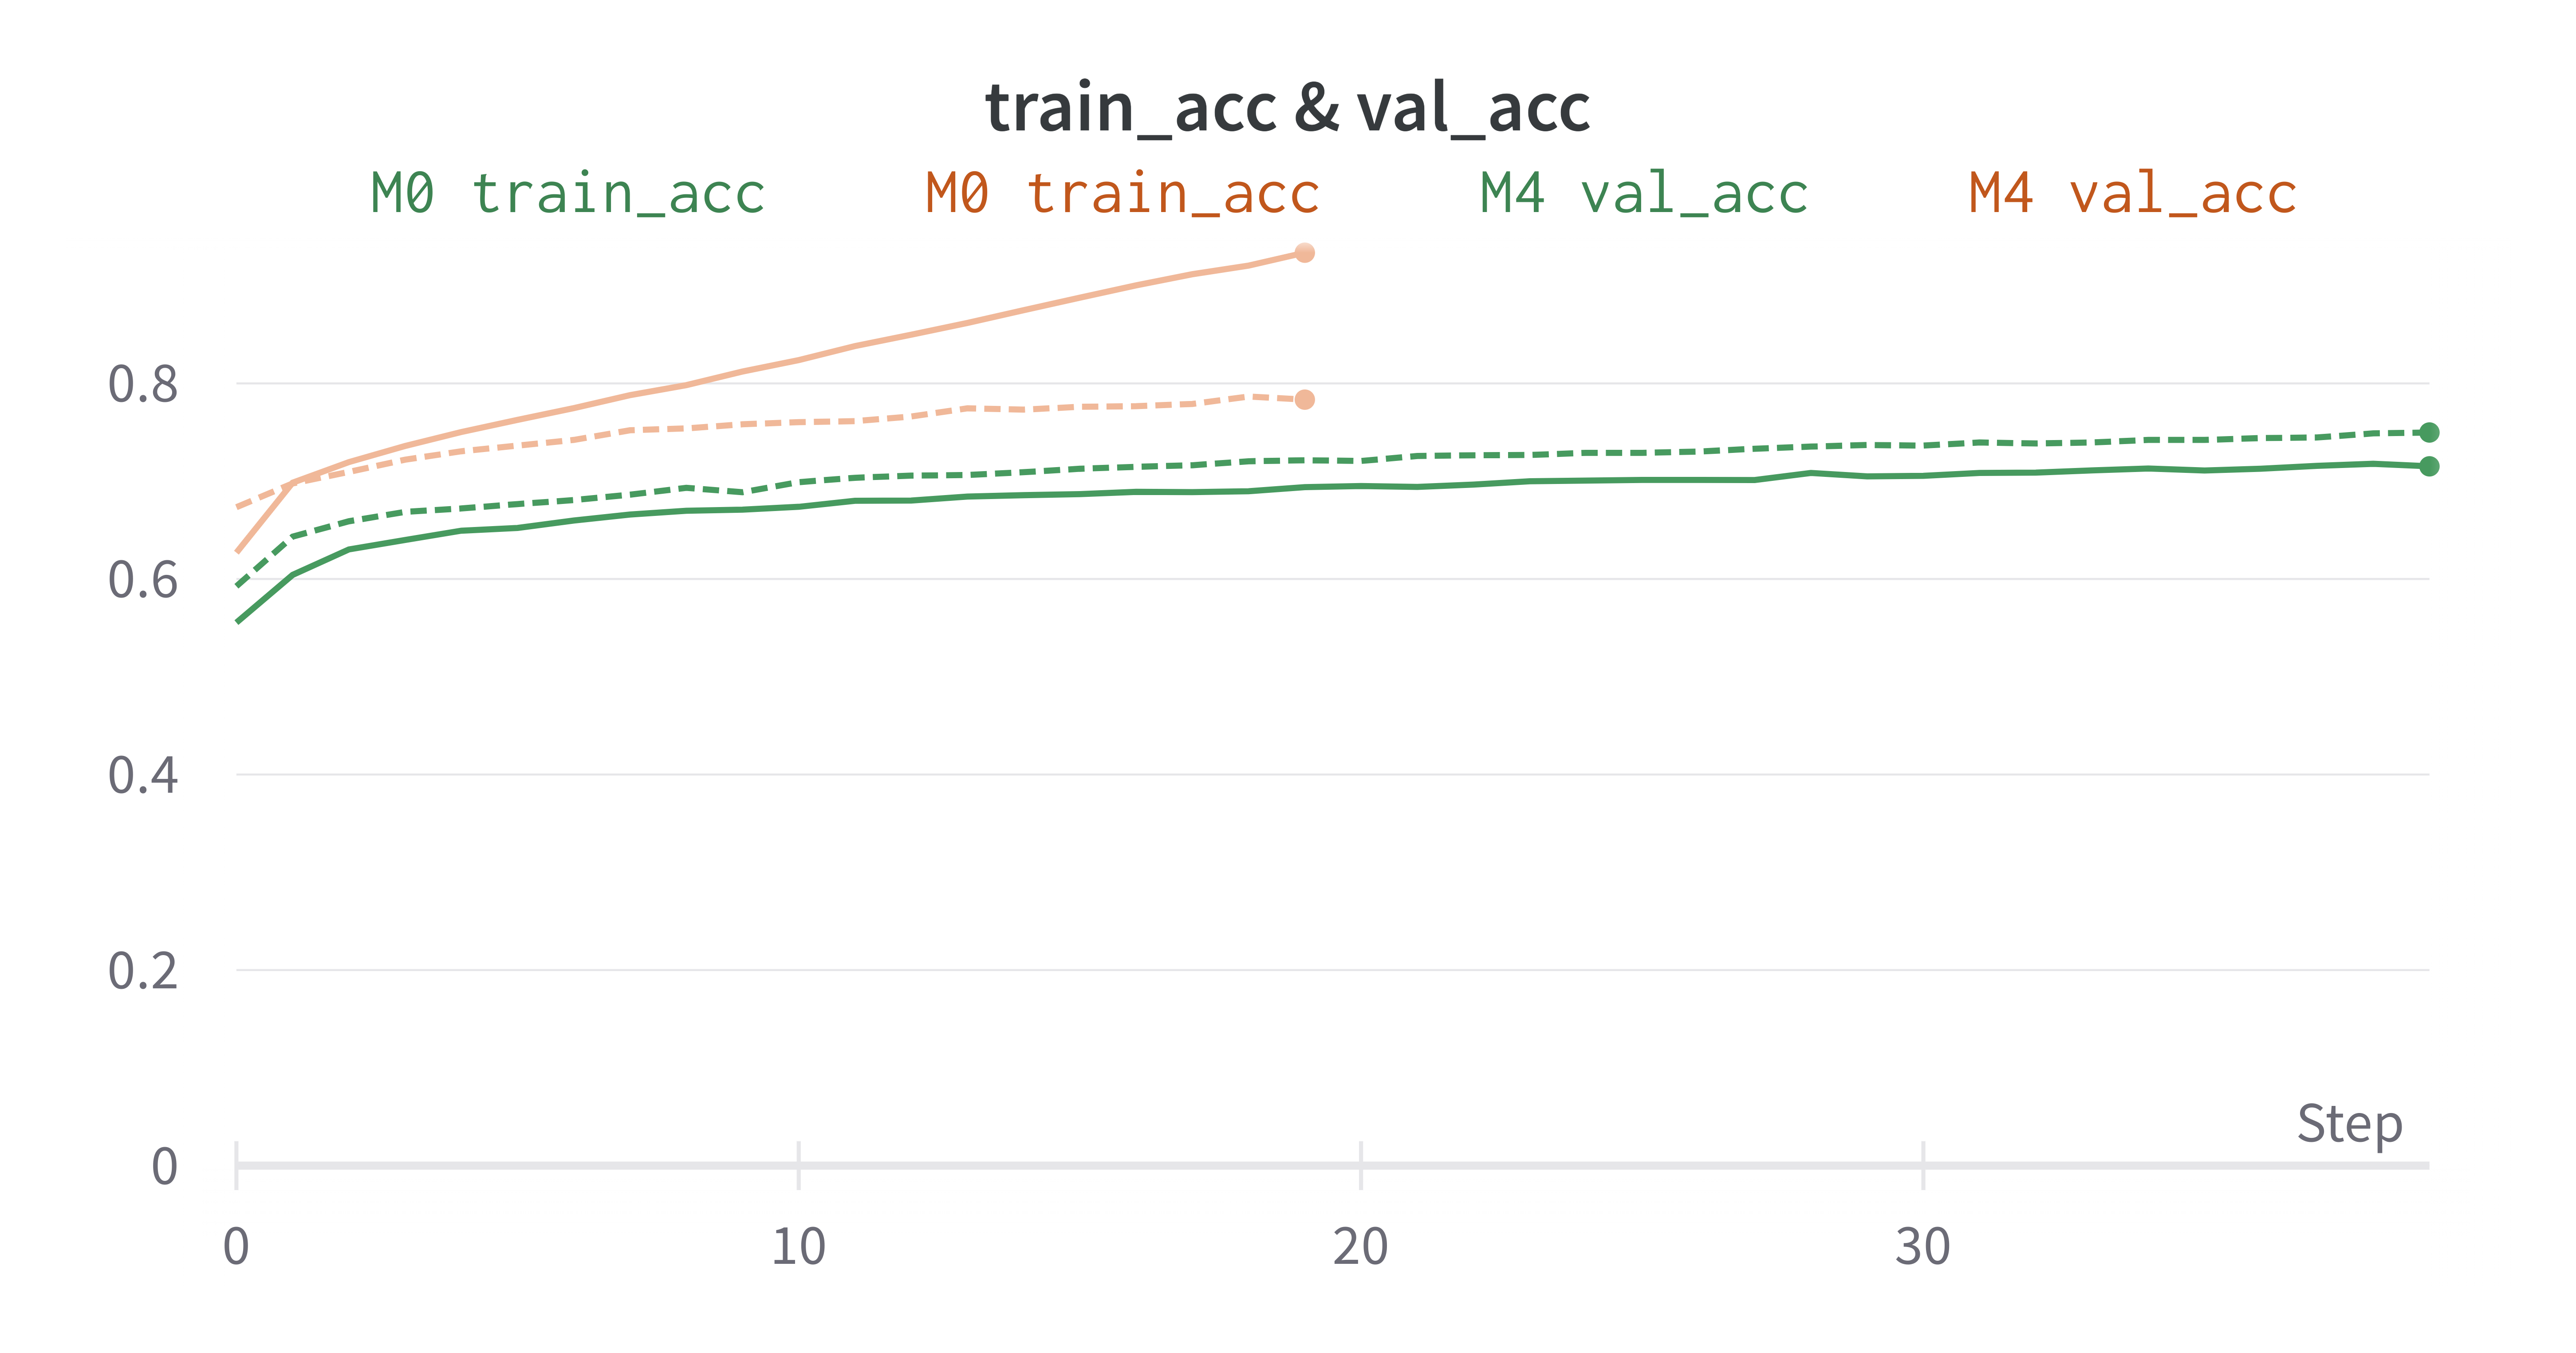
\includegraphics[width=\textwidth]{imatges/results/AccM0M4.png}
\caption[M0 vs. M4, Acc Train and Validation Curves]{\textit{M0 vs. M4, Acc Train and Validation Curves. Illustration by Author}}
{\label{fig:accm0m4}}
\end{figure}

\newpage


\subsection{M1 against M5}

\begin{figure}[H]
\centering
    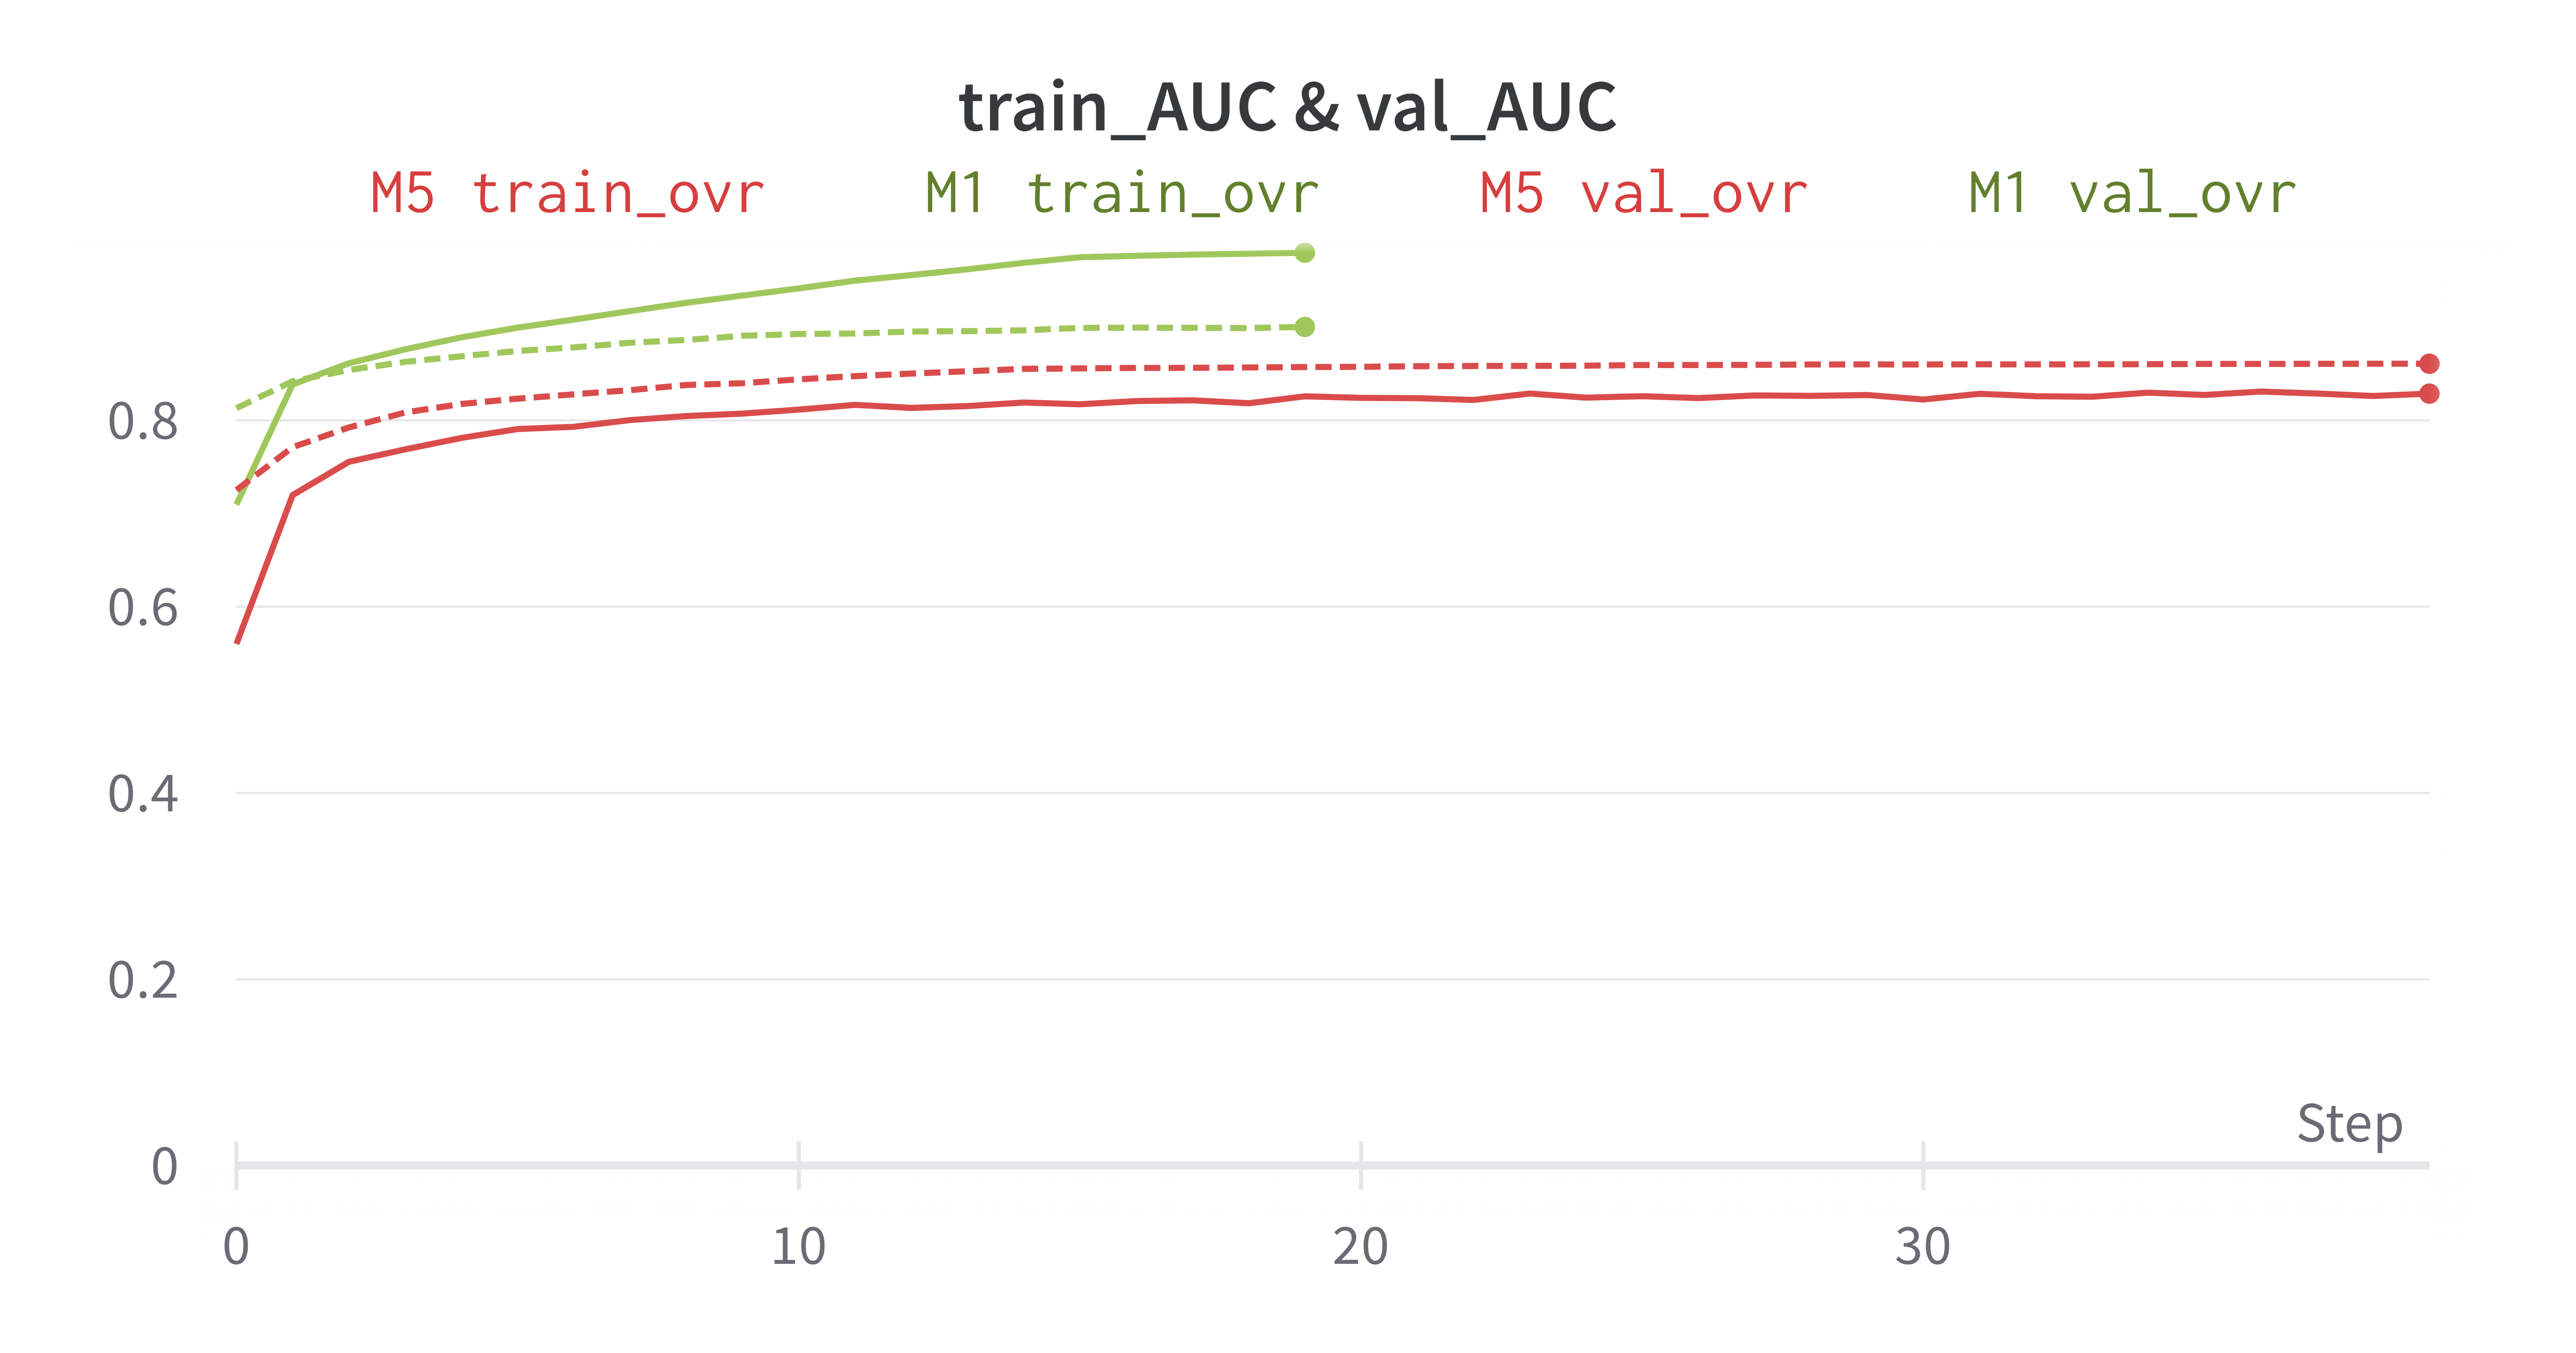
\includegraphics[width=\textwidth]{imatges/results/AUCM1M5.png}
\caption[M1 vs. M5, AUC Train and Validation Curves]{\textit{M1 vs. M5, AUC Train and Validation Curves. Illustration by Author}}
{\label{fig:aucm0m4}}
\end{figure}


\begin{figure}[H]
\centering
    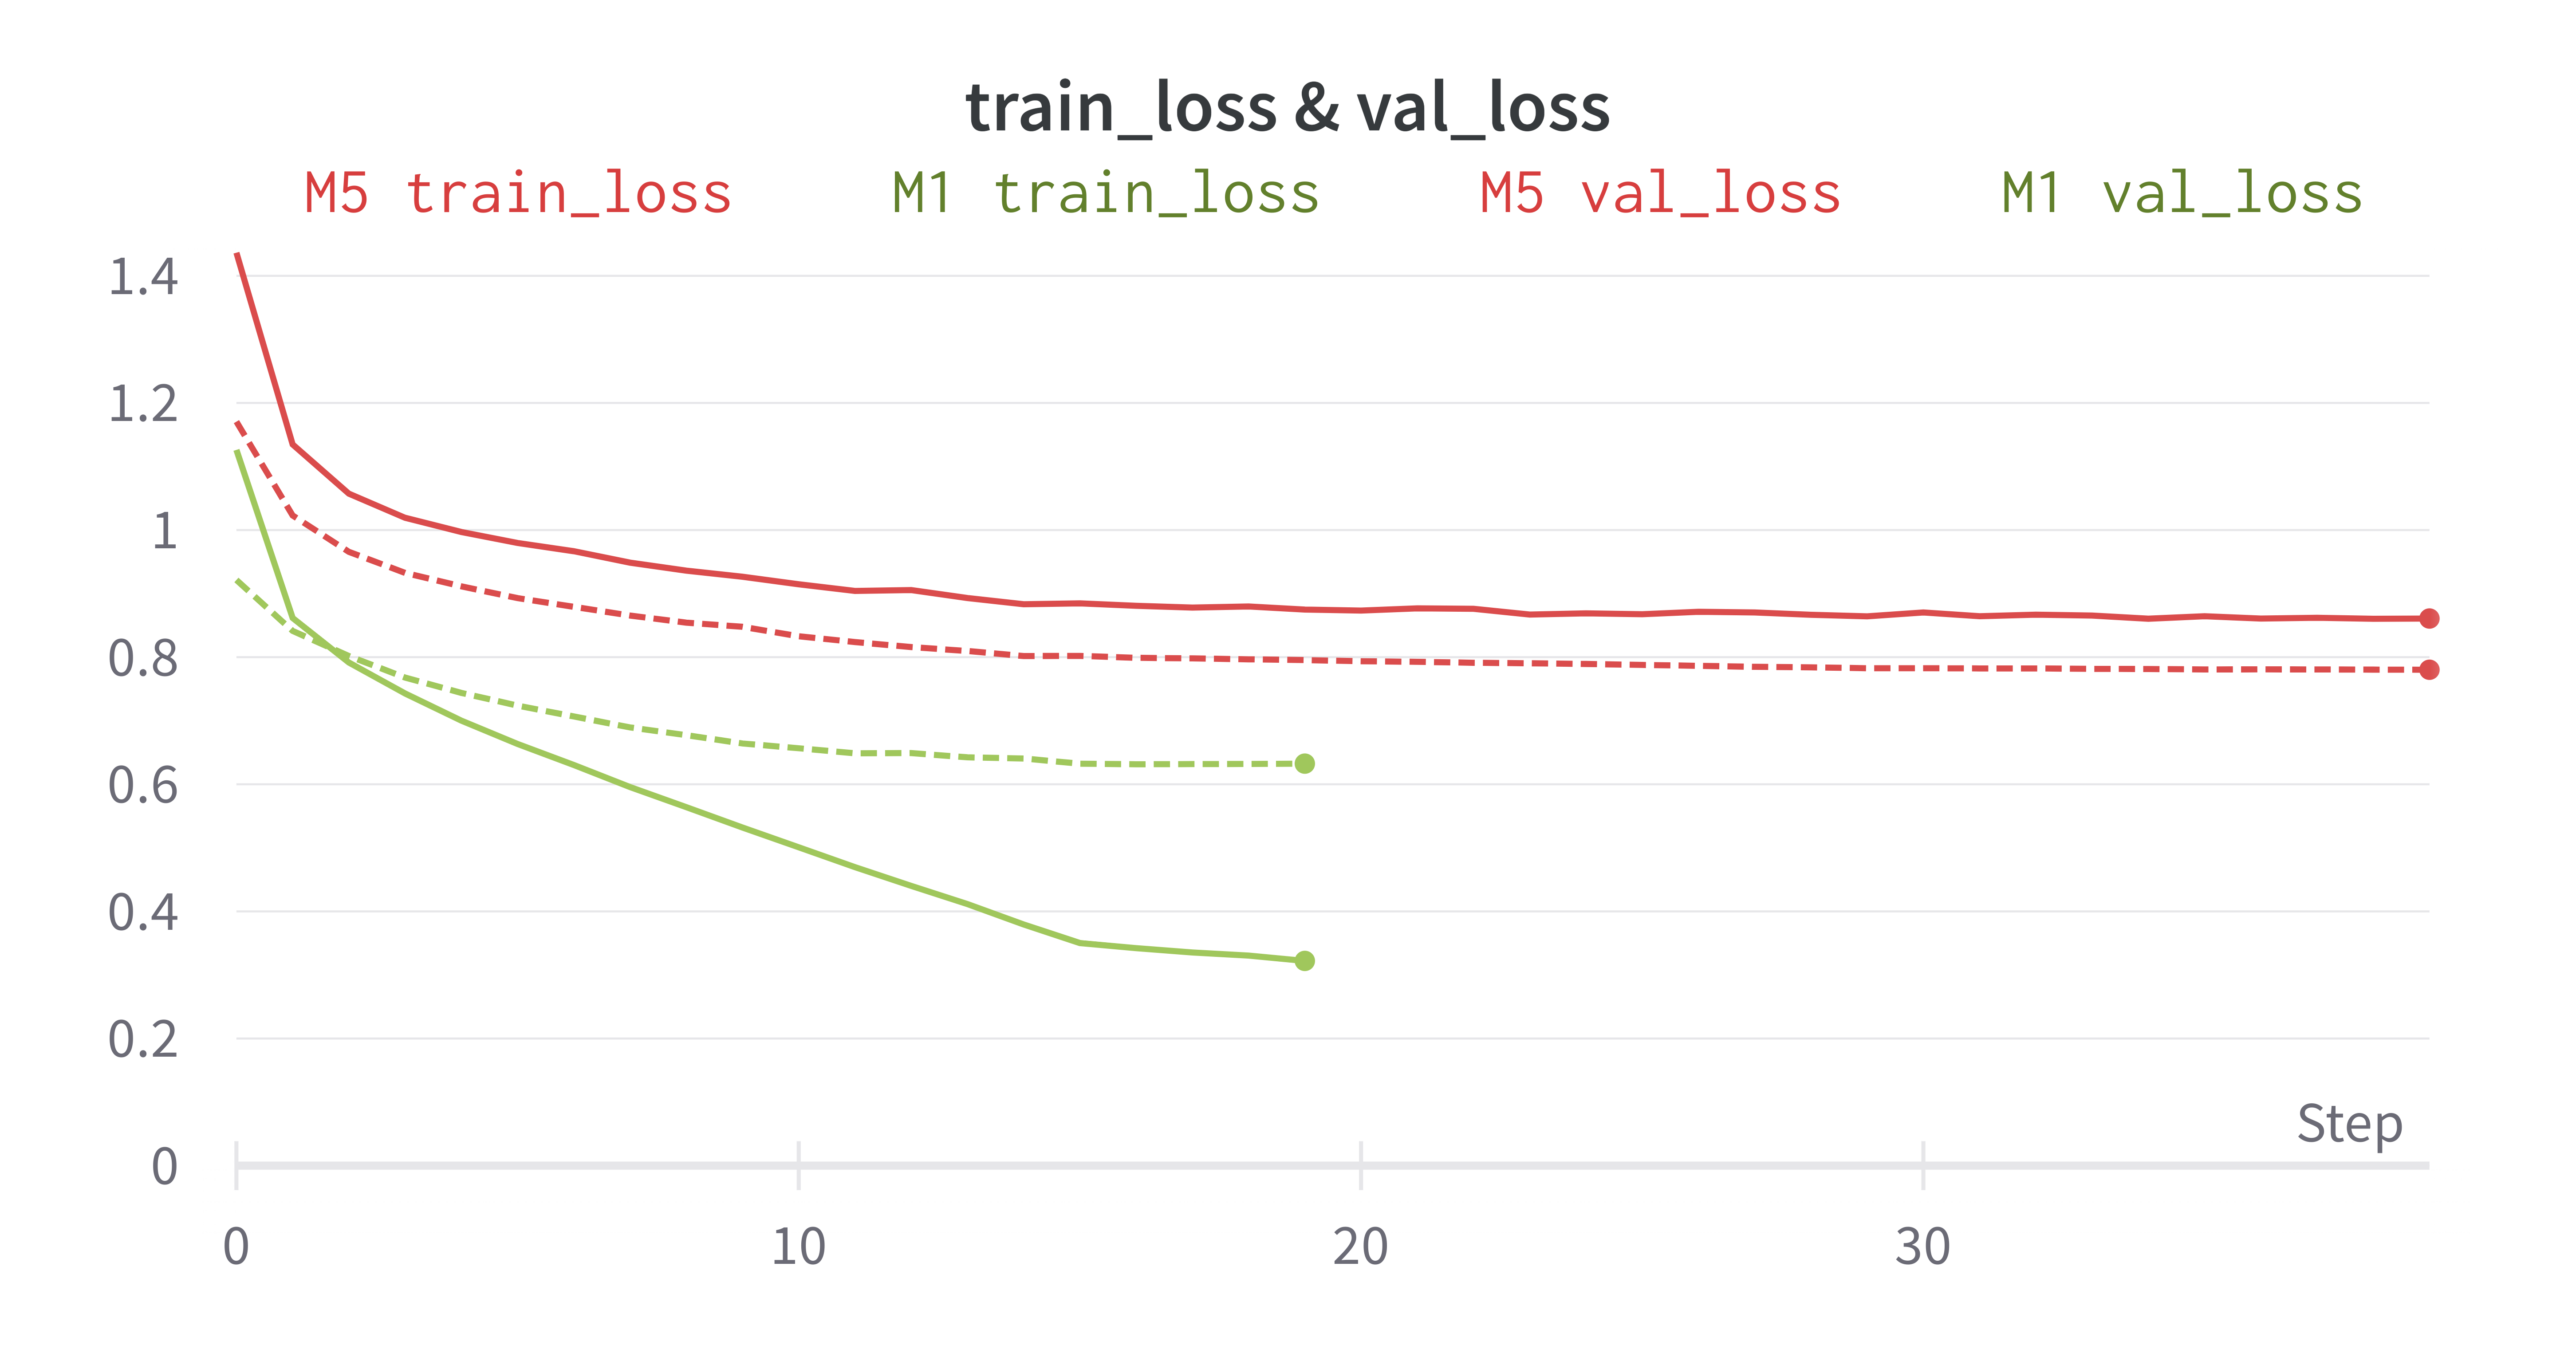
\includegraphics[width=\textwidth]{imatges/results/LossM1M5.png}
\caption[M1 vs. M5, Loss Train and Validation Curves]{\textit{M1 vs. M5, Loss Train and Validation Curves. Illustration by Author}}
{\label{fig:lossm0m4}}
\end{figure}

\newpage

\begin{figure}[H]
\centering
    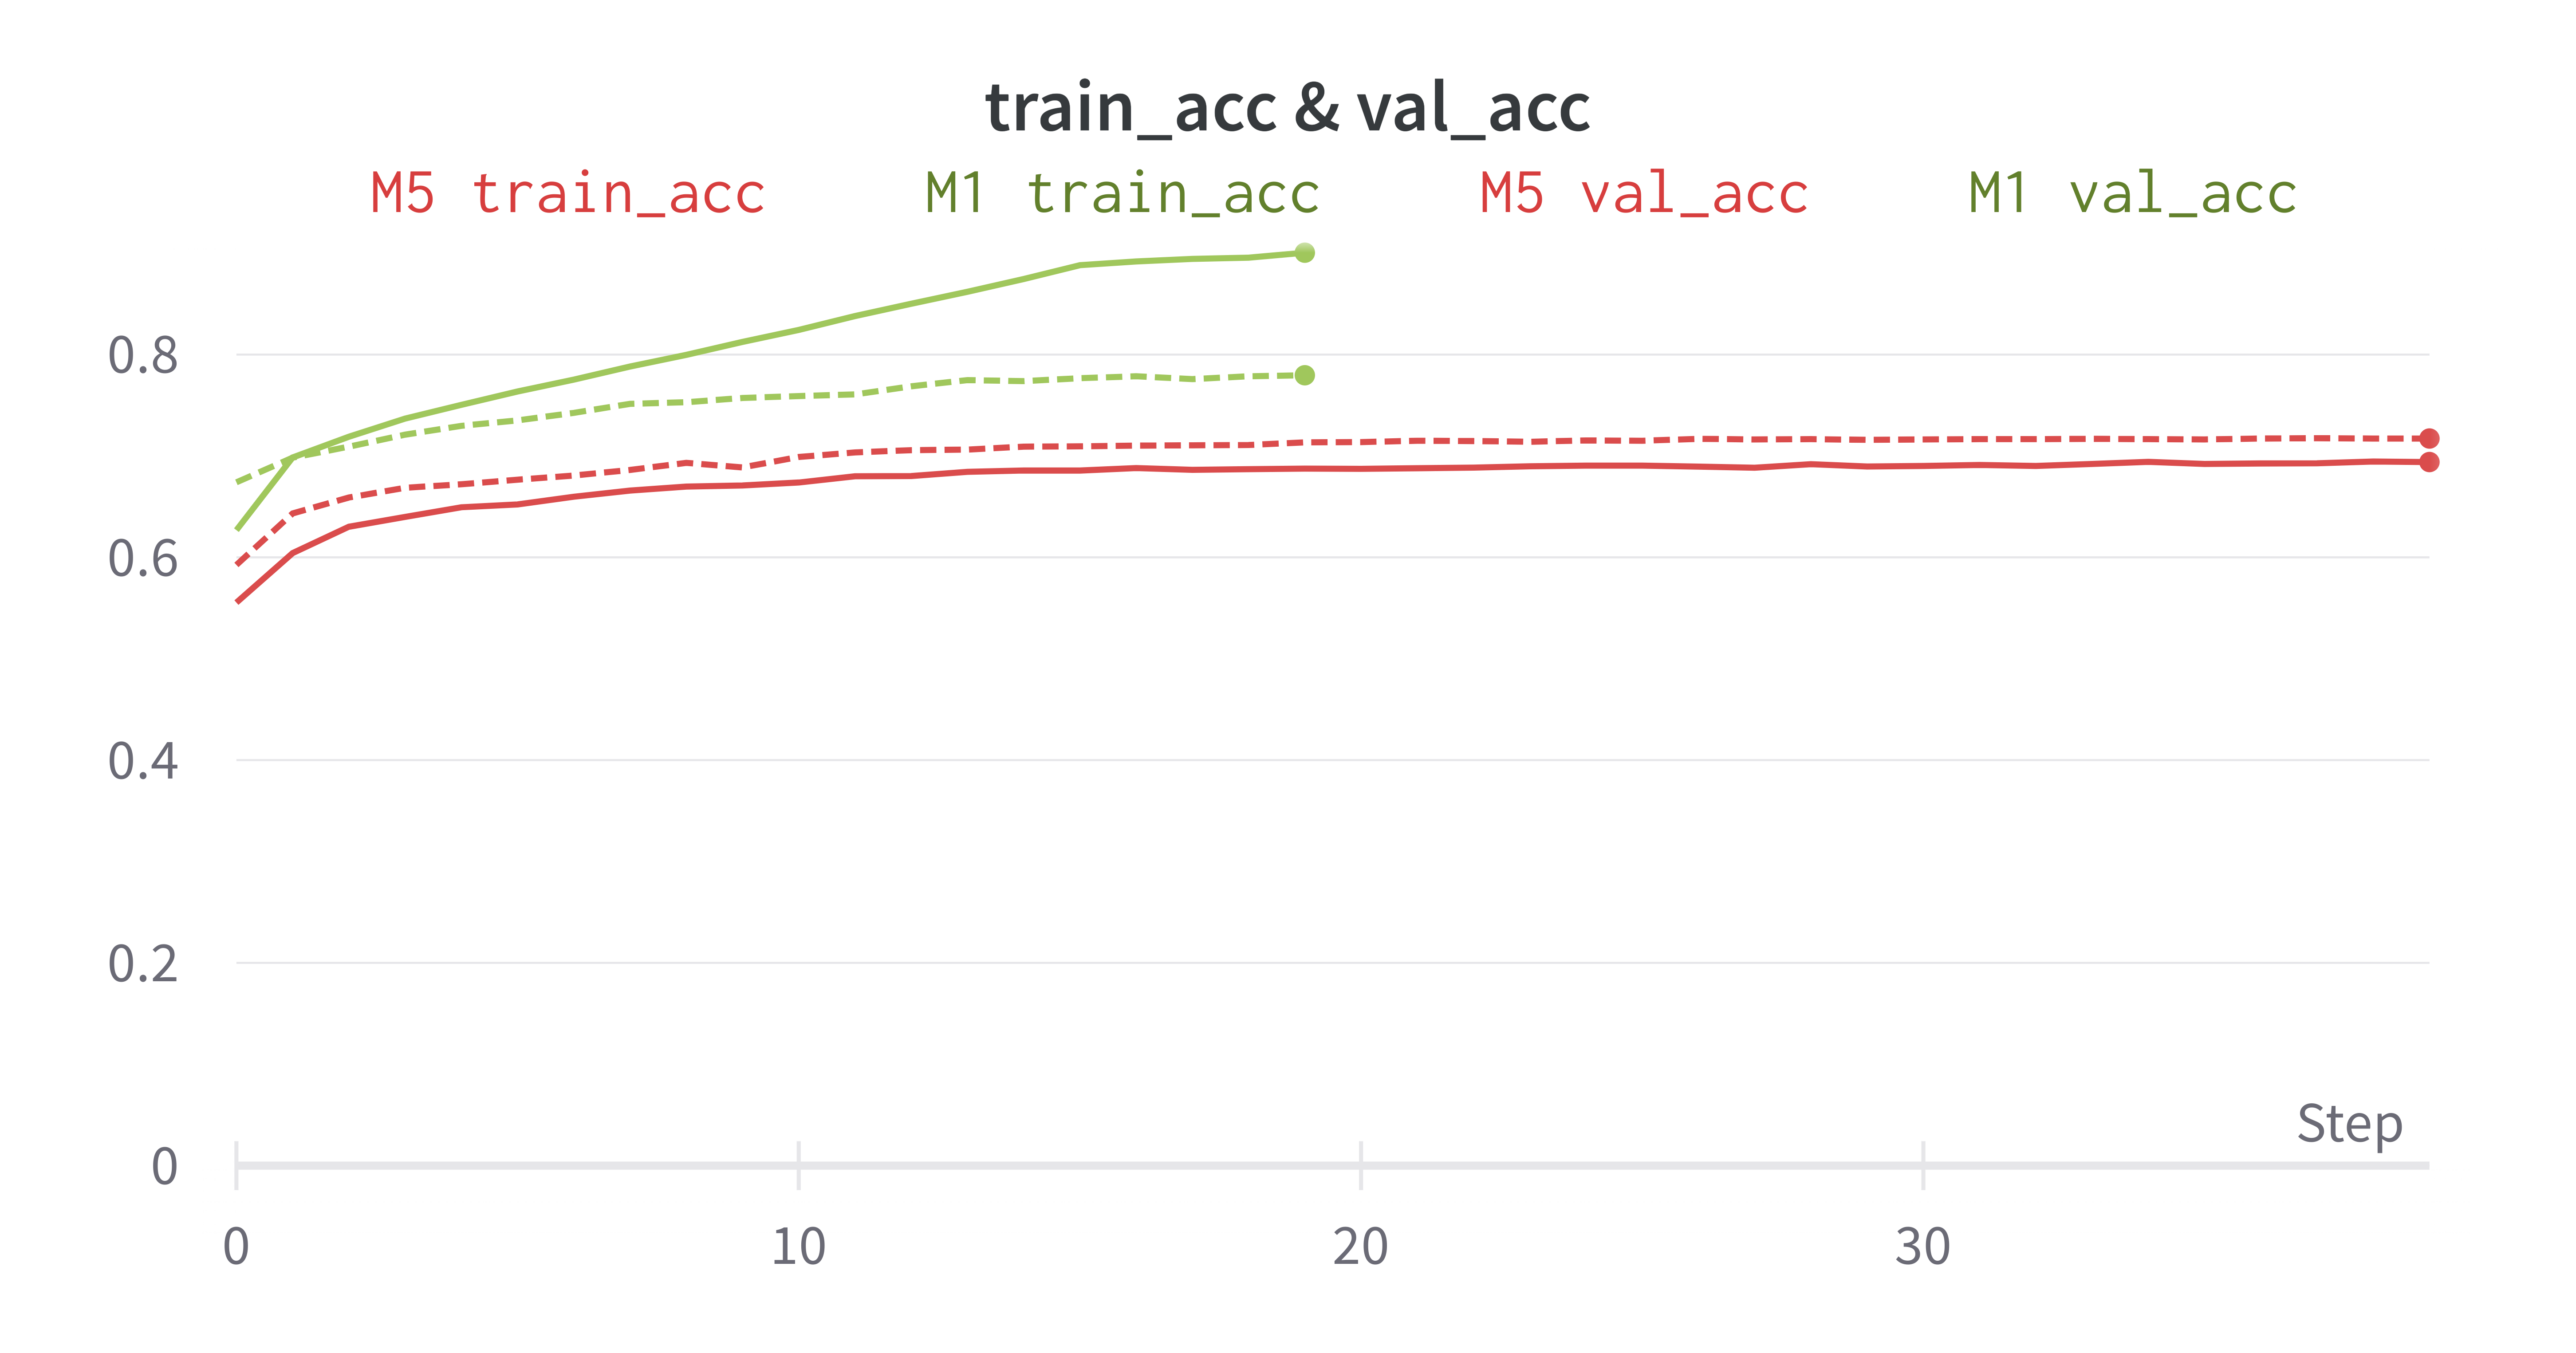
\includegraphics[width=\textwidth]{imatges/results/AccM1M5.png}
\caption[M1 vs. M5, Acc Train and Validation Curves]{\textit{M1 vs. M5, Acc Train and Validation Curves. Illustration by Author}}
{\label{fig:accm0m4}}
\end{figure}


\subsection{M2 against M6}

\begin{figure}[H]
\centering
    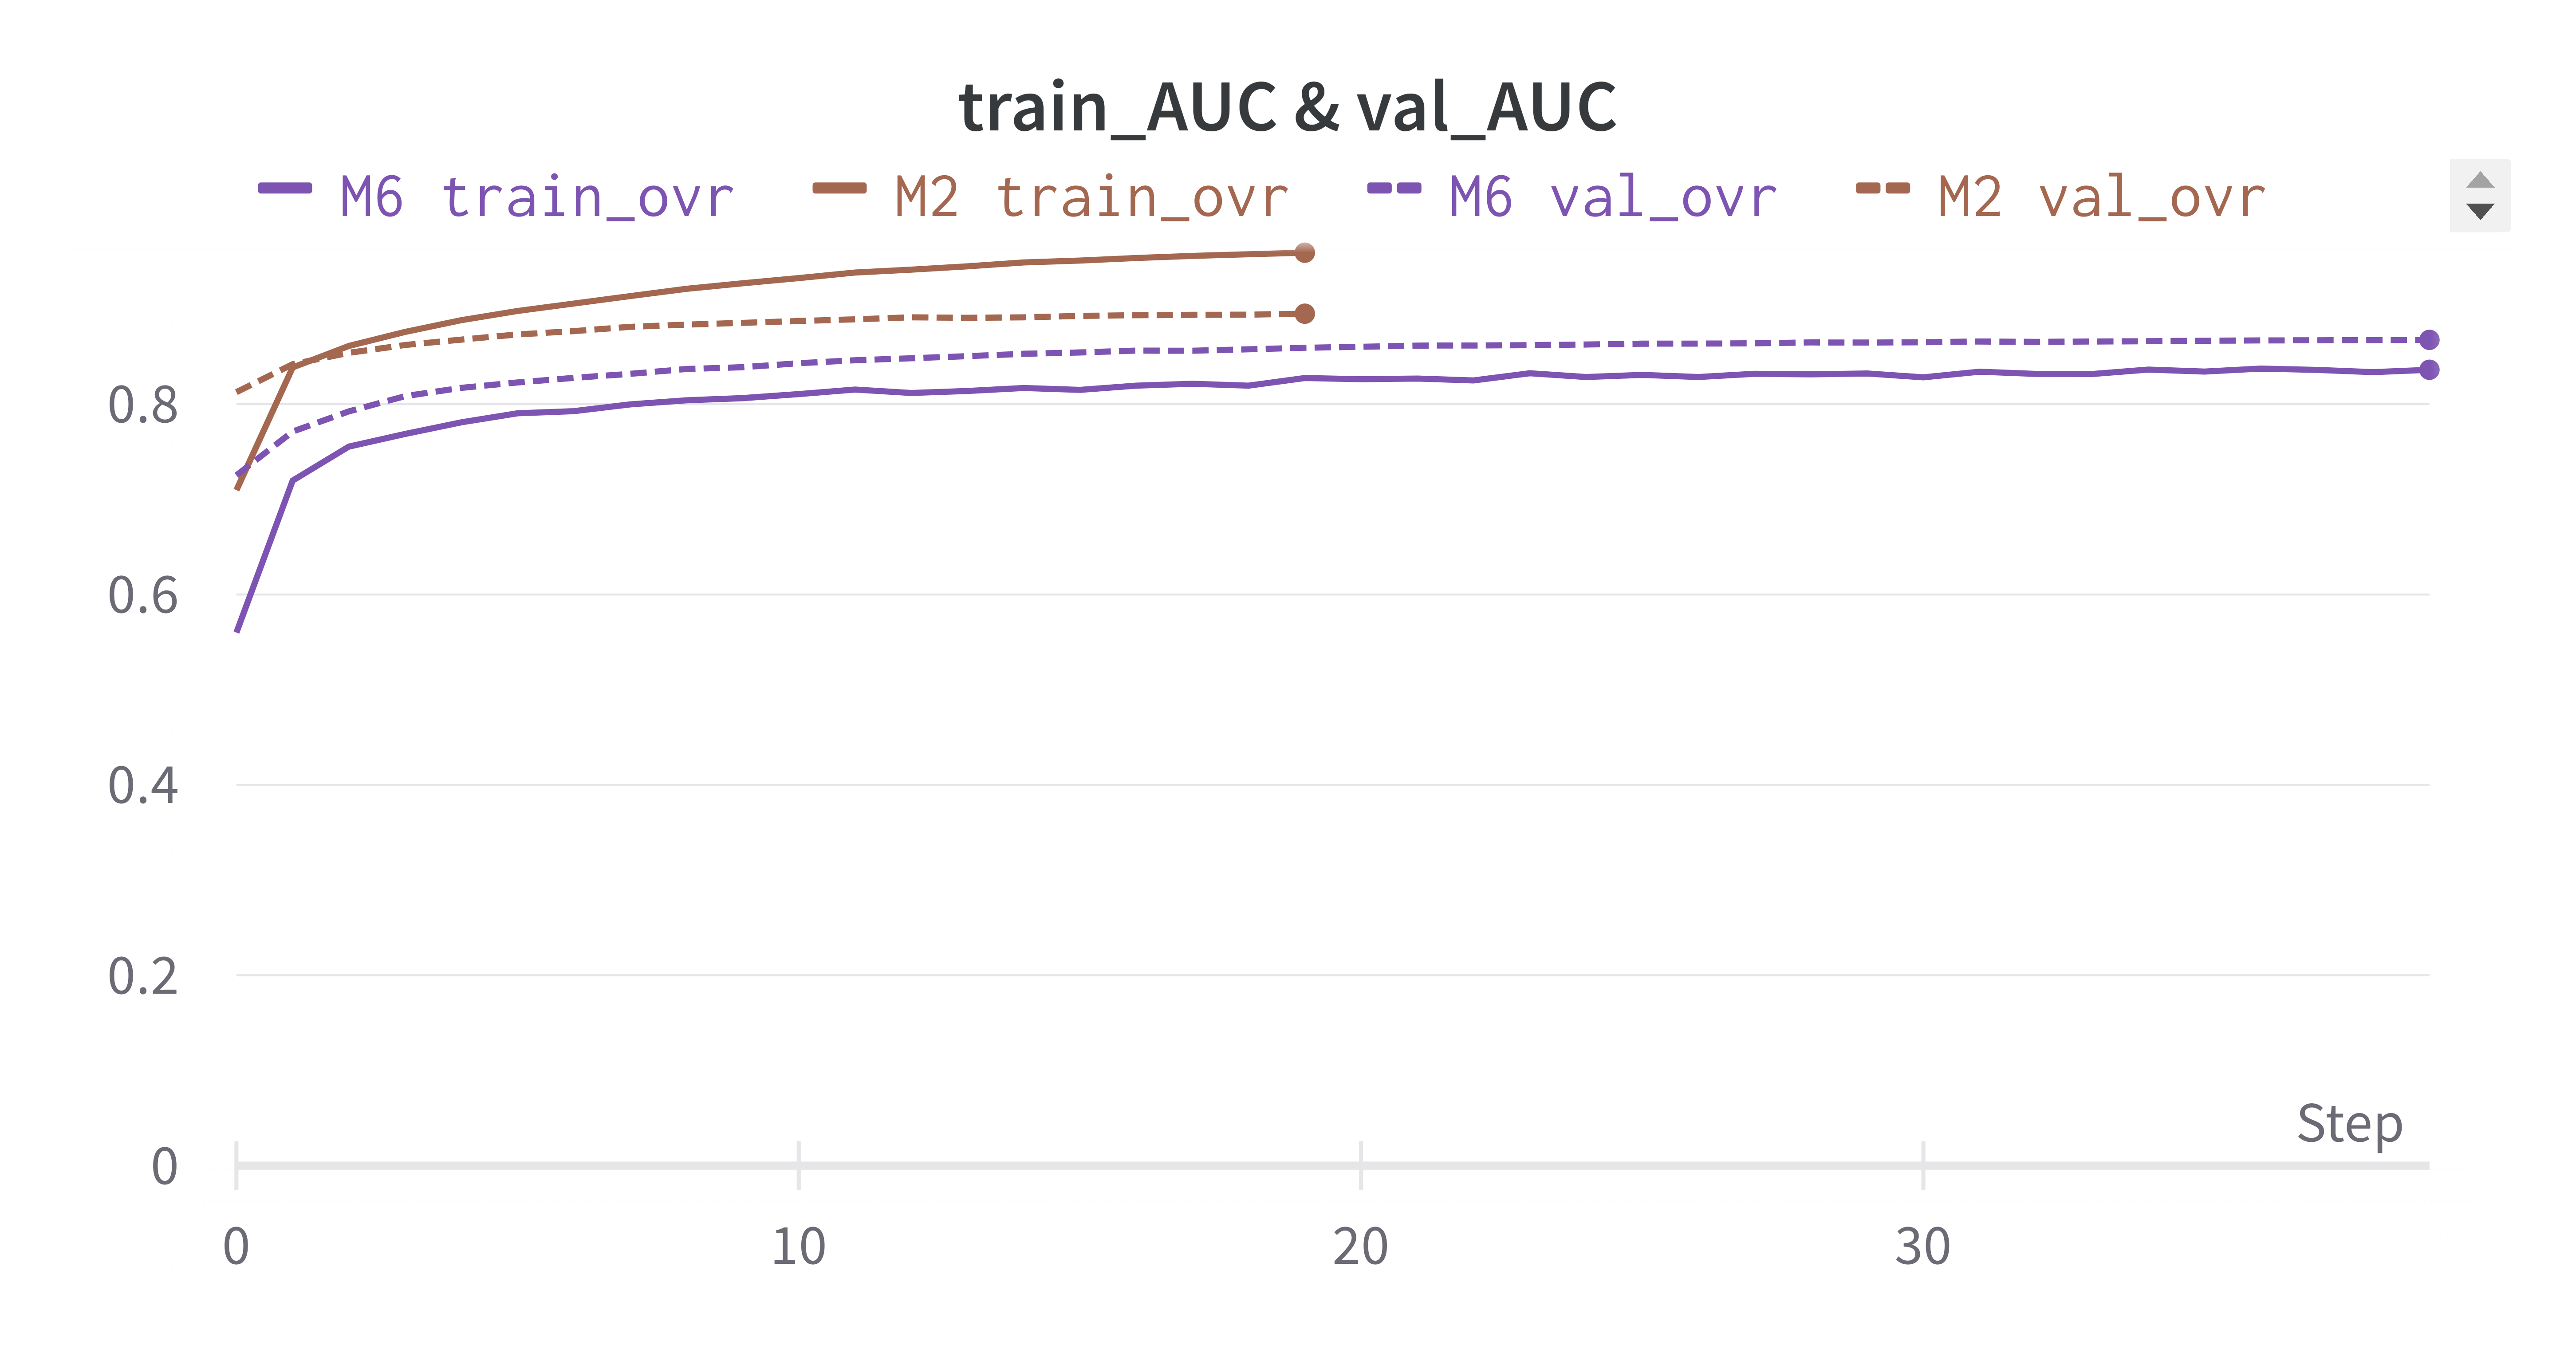
\includegraphics[width=\textwidth]{imatges/results/AUCM2M6.png}
\caption[M2 vs. M6, AUC Train and Validation Curves]{\textit{M2 vs. M6, AUC Train and Validation Curves. Illustration by Author}}
{\label{fig:aucm0m4}}
\end{figure}

\newpage

\begin{figure}[H]
\centering
    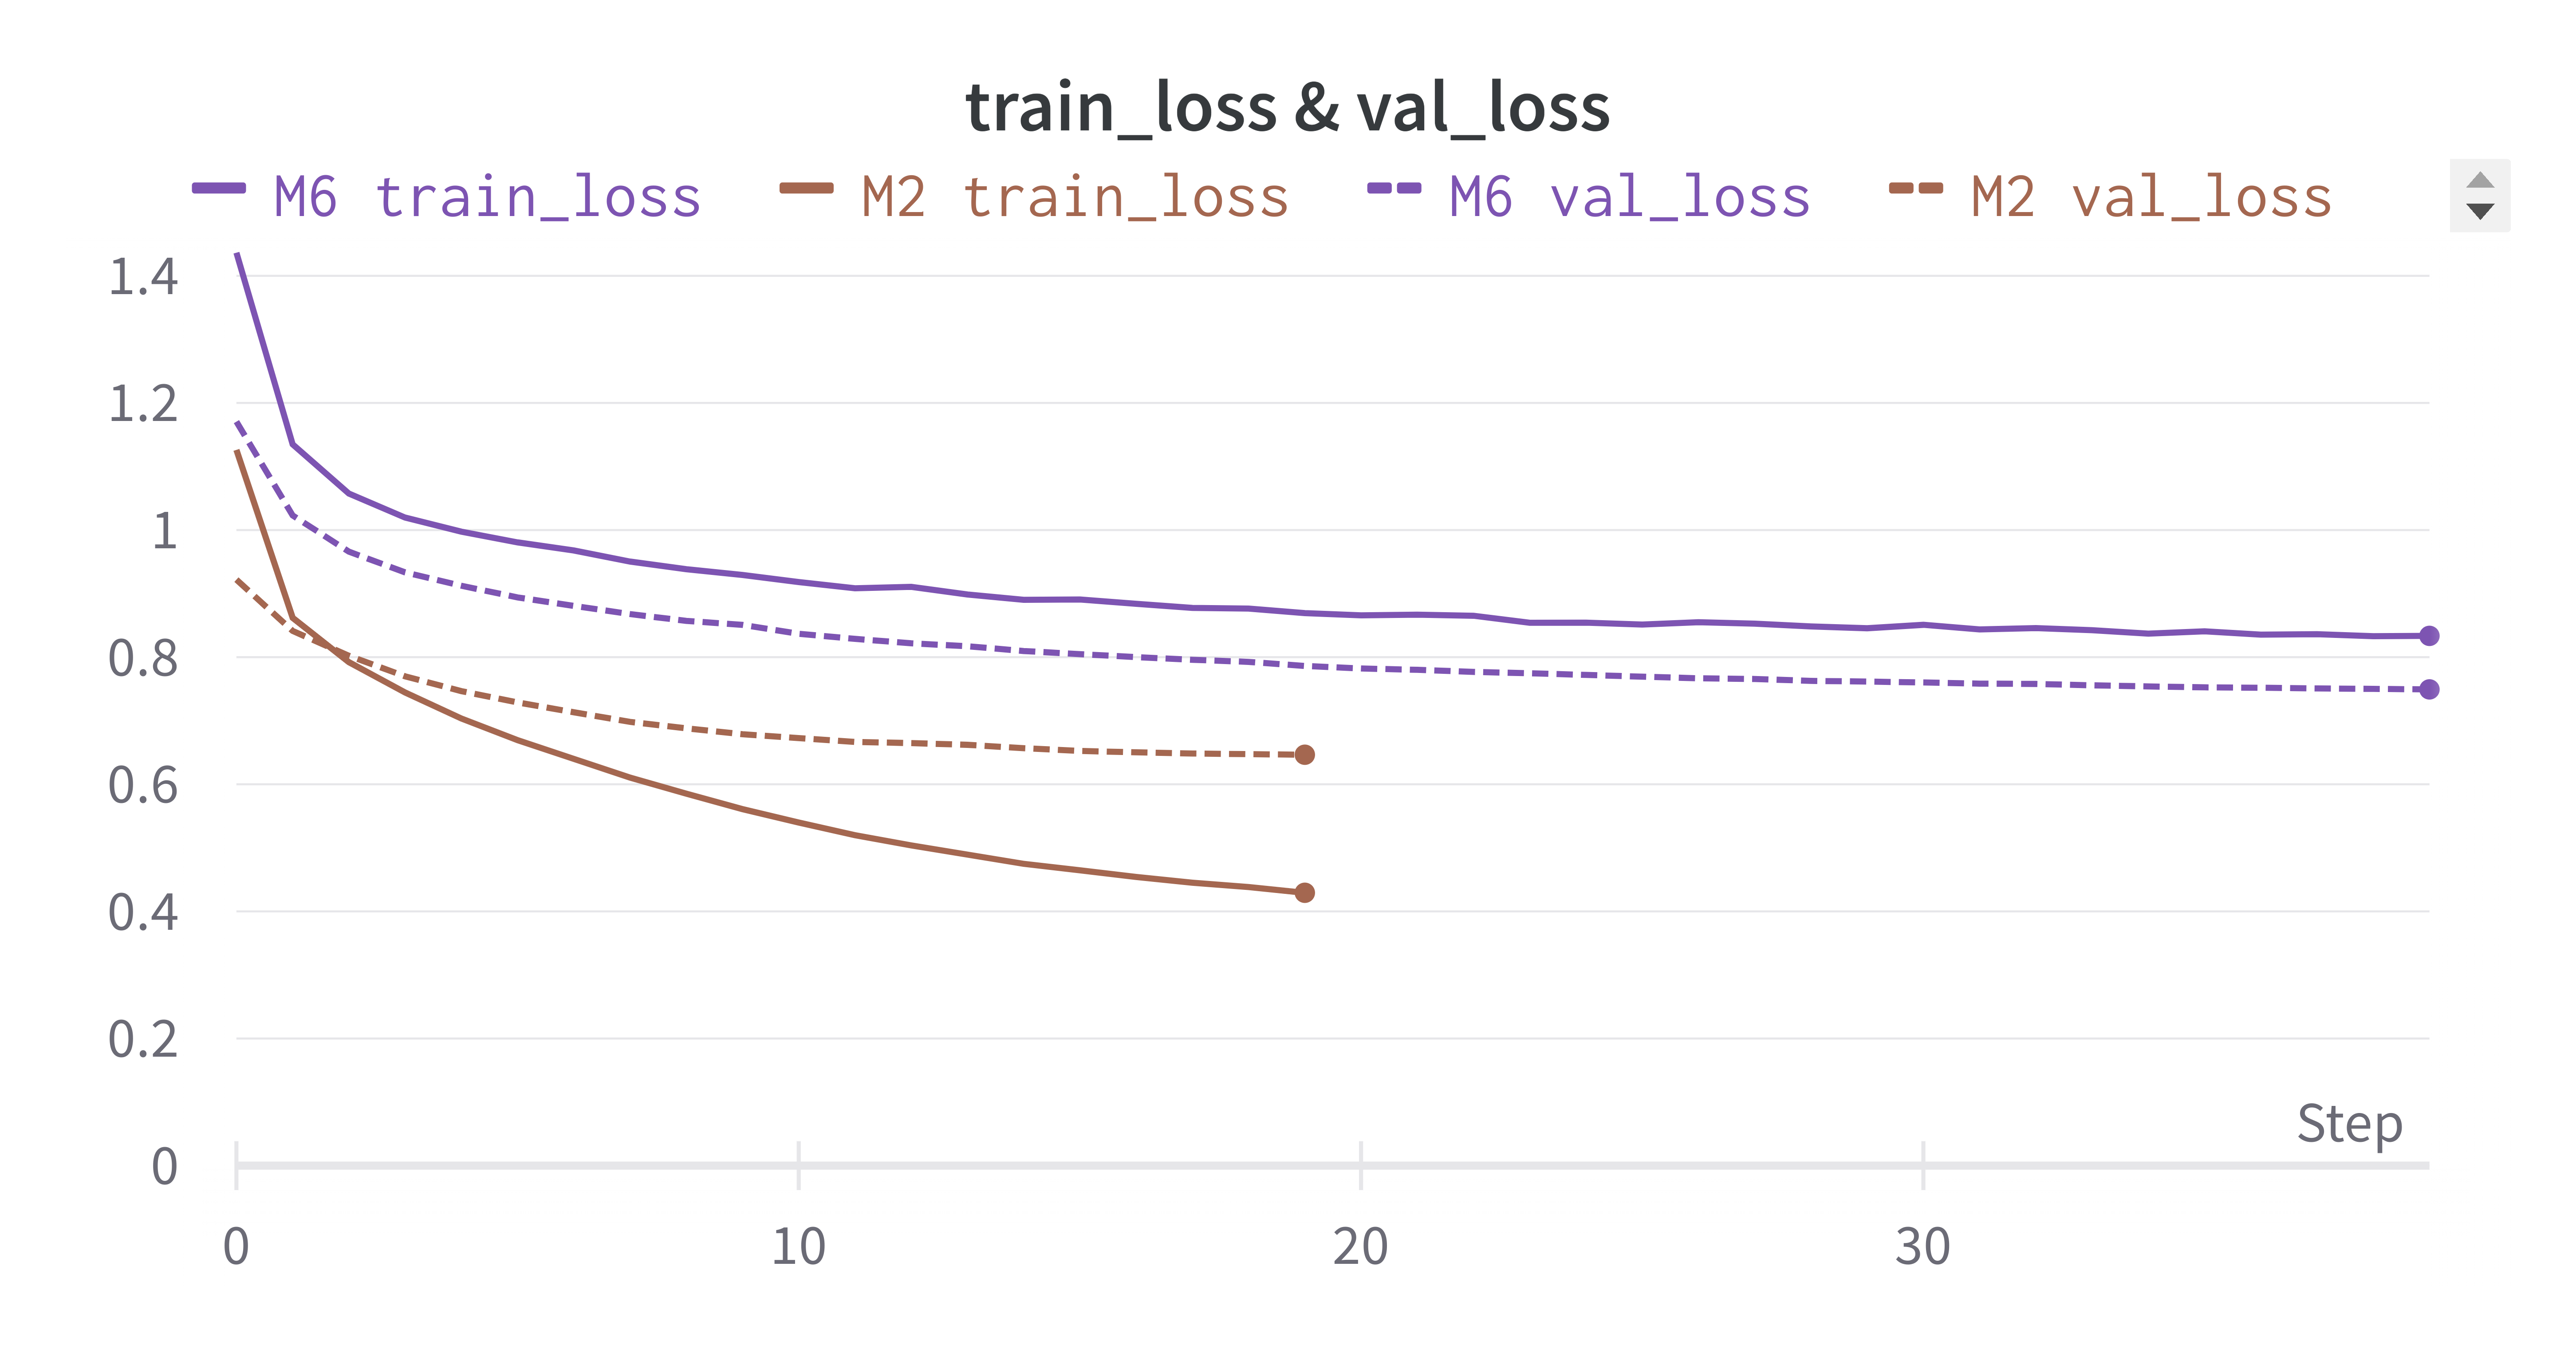
\includegraphics[width=\textwidth]{imatges/results/LossM2M6.png}
\caption[M2 vs. M6, Loss Train and Validation Curves]{\textit{M2 vs. M6, Loss Train and Validation Curves. Illustration by Author}}
{\label{fig:lossm0m4}}
\end{figure}


\begin{figure}[H]
\centering
    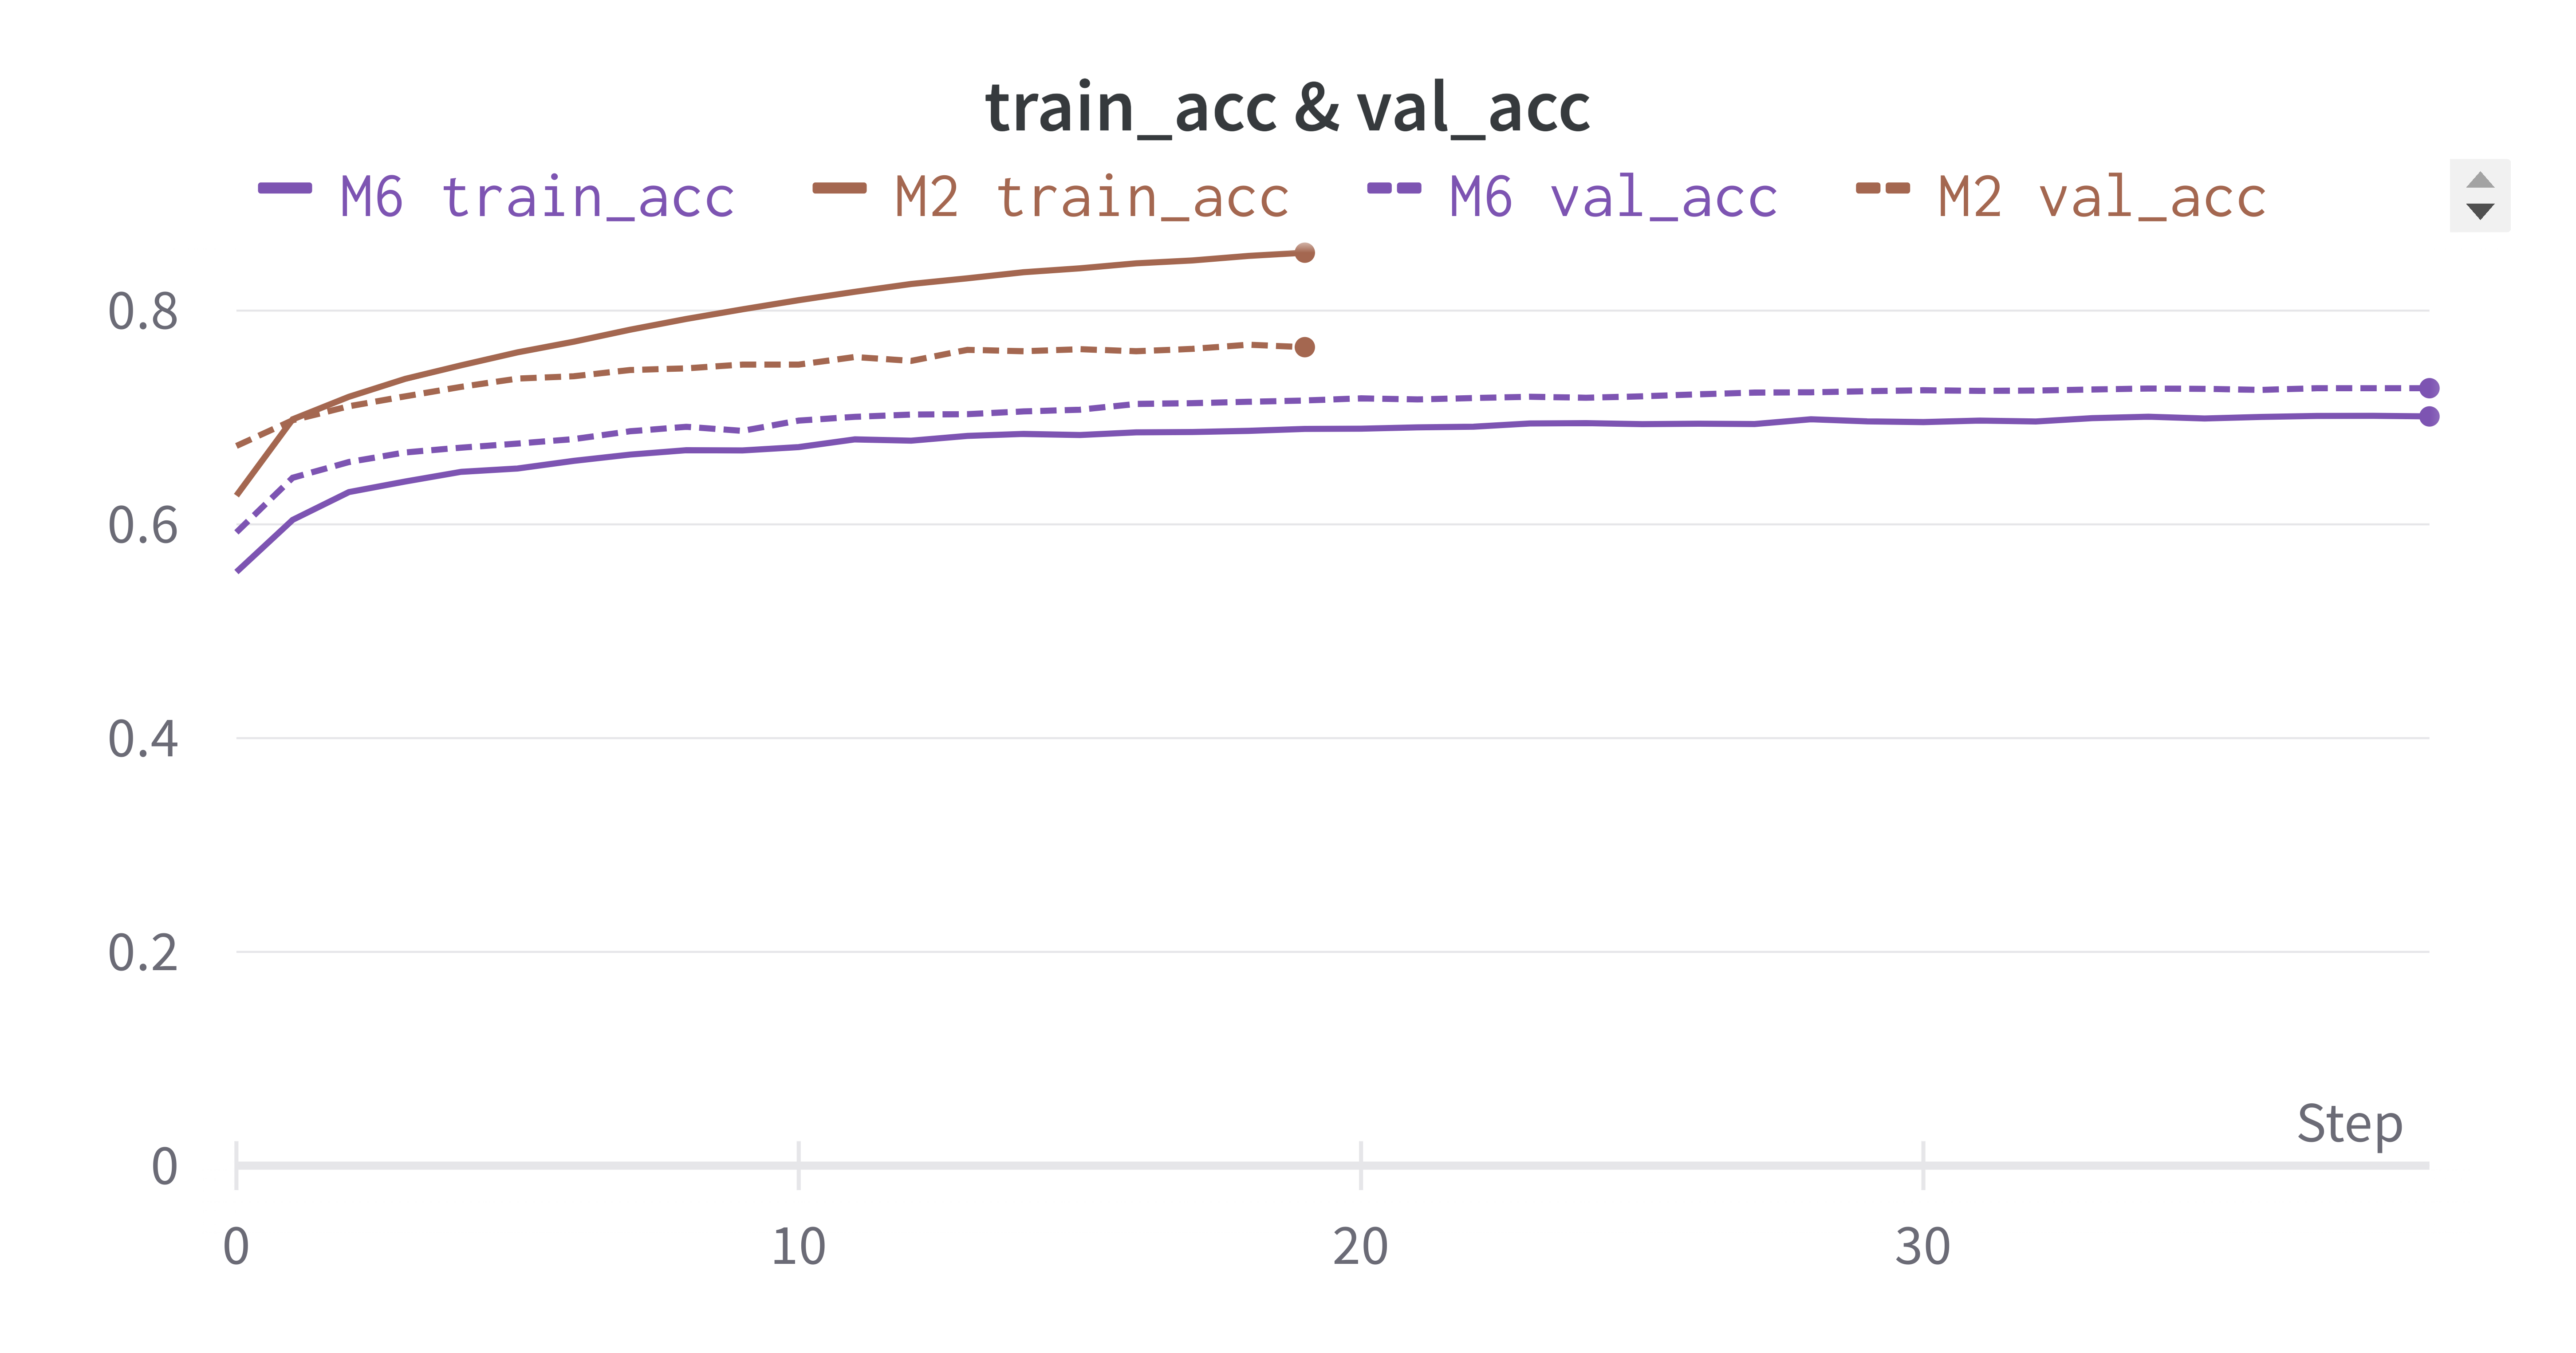
\includegraphics[width=\textwidth]{imatges/results/AccM2M6.png}
\caption[M2 vs. M6, Acc Train and Validation Curves]{\textit{M2 vs. M6, Acc Train and Validation Curves. Illustration by Author}}
{\label{fig:accm0m4}}
\end{figure}

\newpage

\subsection{M3 against M7}

\begin{figure}[H]
\centering
    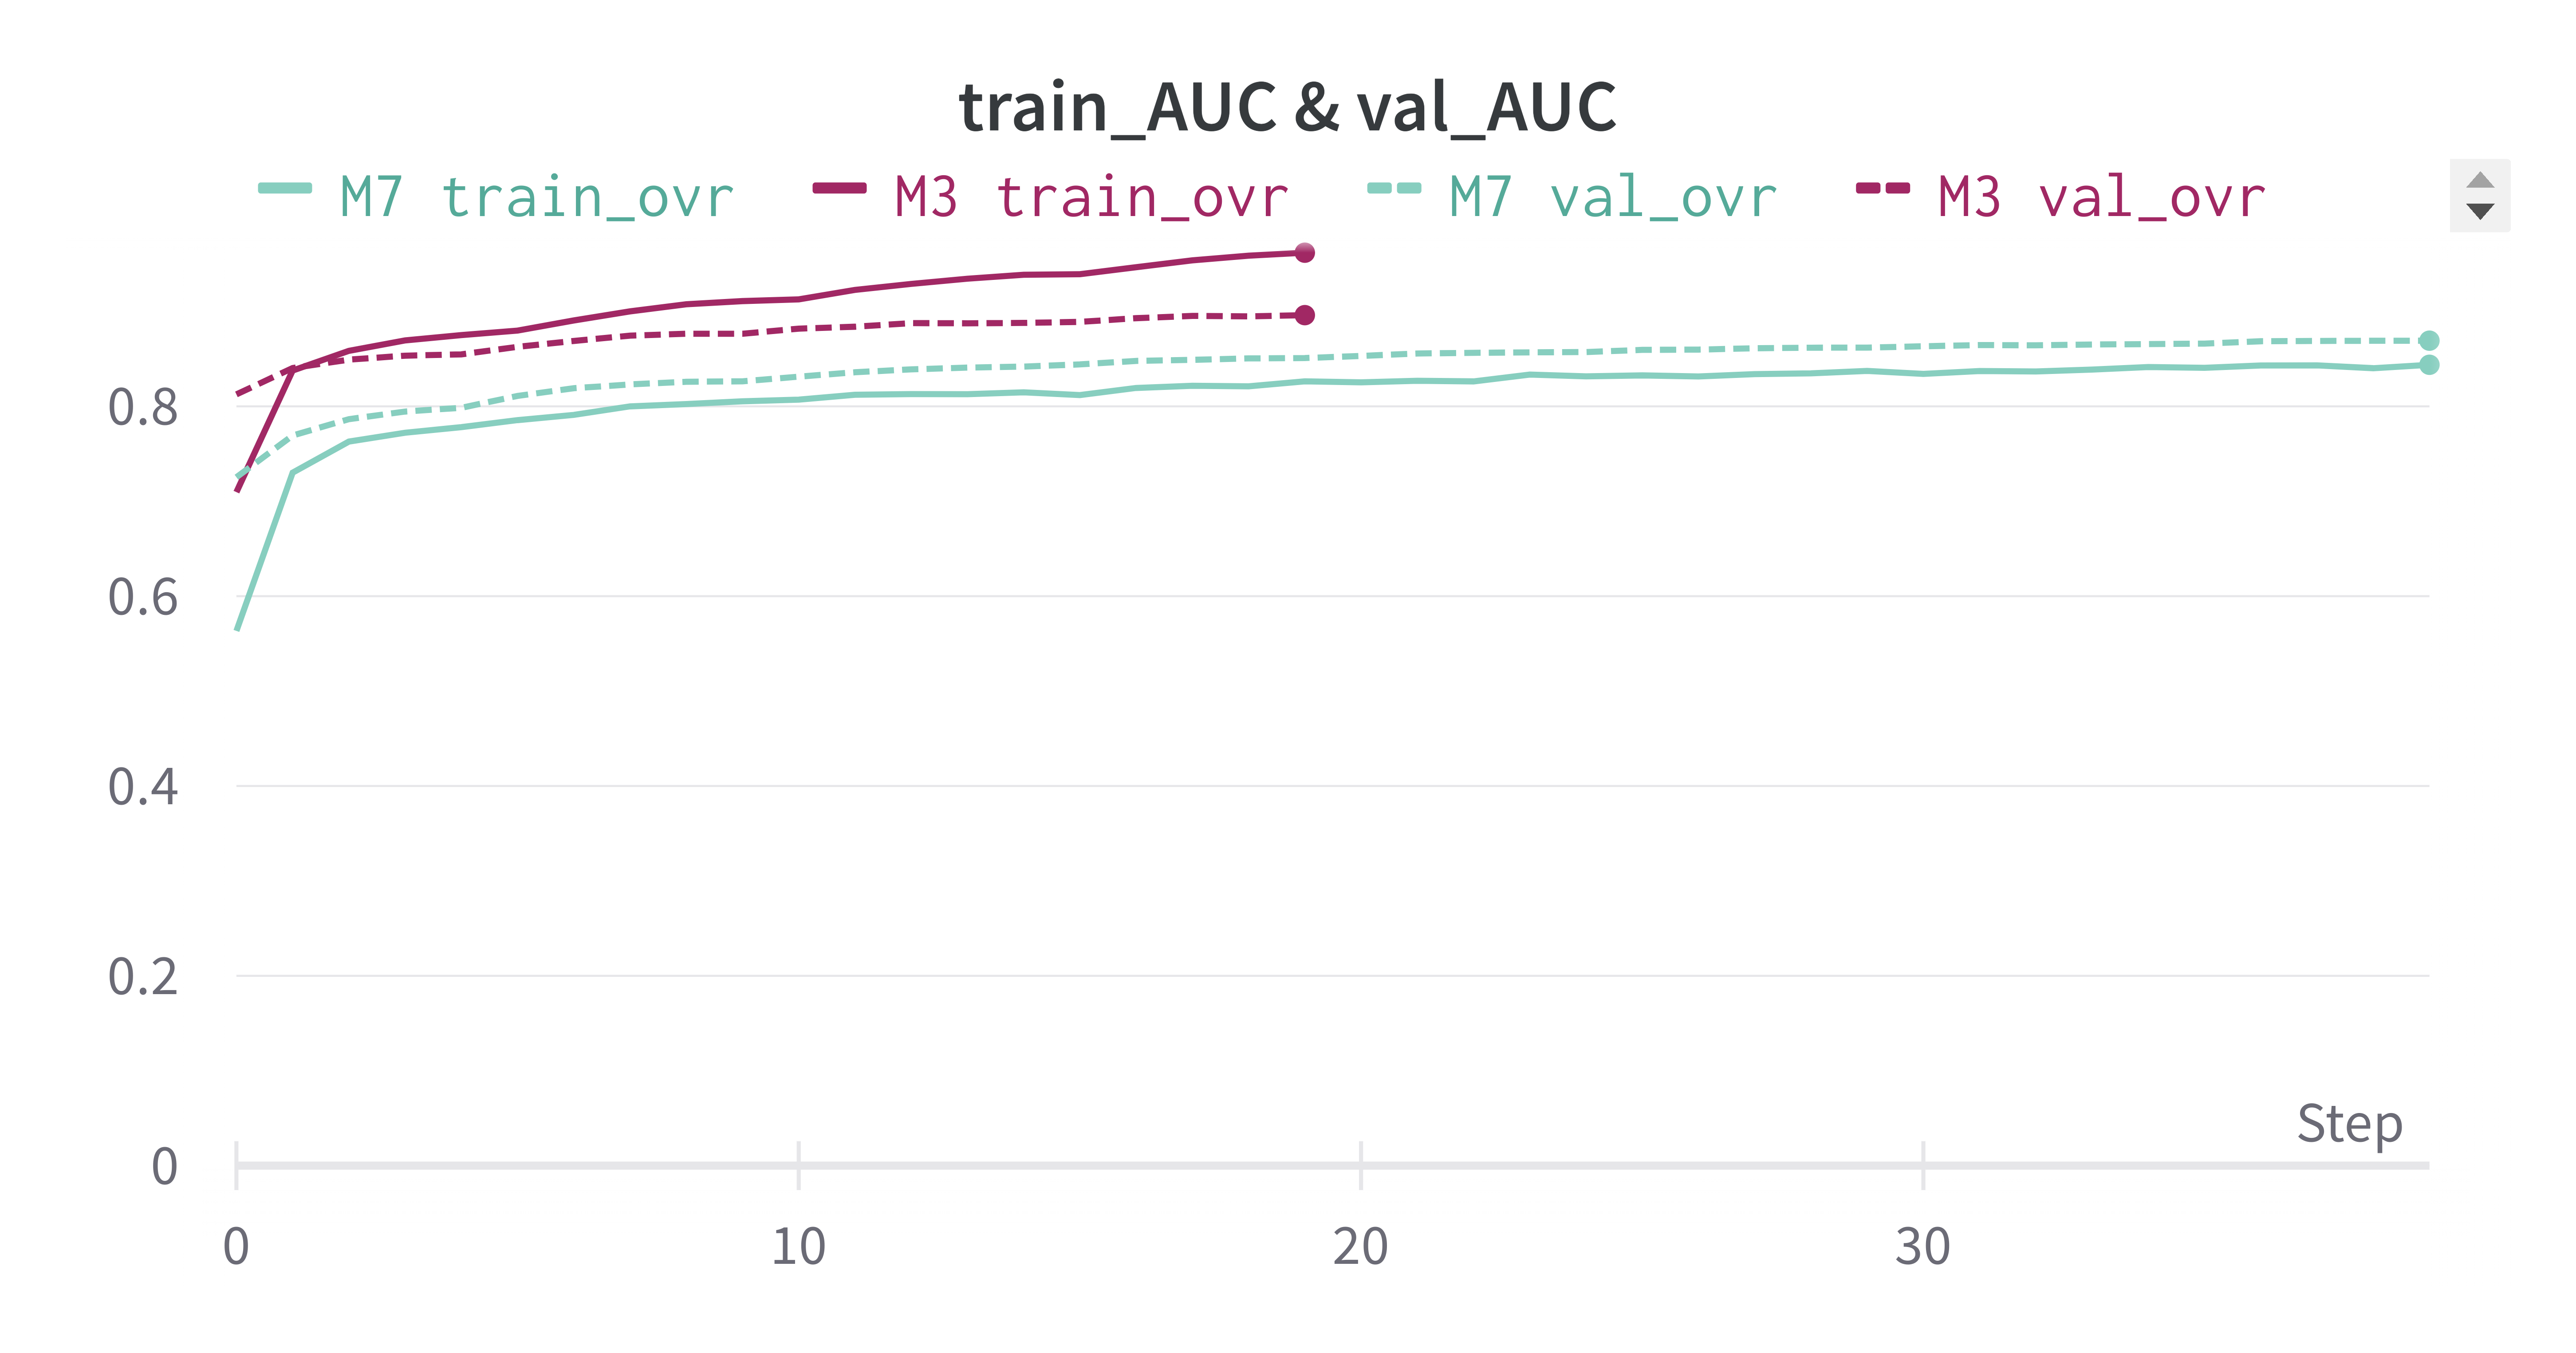
\includegraphics[width=\textwidth]{imatges/results/AUCM3M7.png}
\caption[M3 vs. M7, AUC Train and Validation Curves]{\textit{M3 vs. M7, AUC Train and Validation Curves. Illustration by Author}}
{\label{fig:aucm0m4}}
\end{figure}


\begin{figure}[H]
\centering
    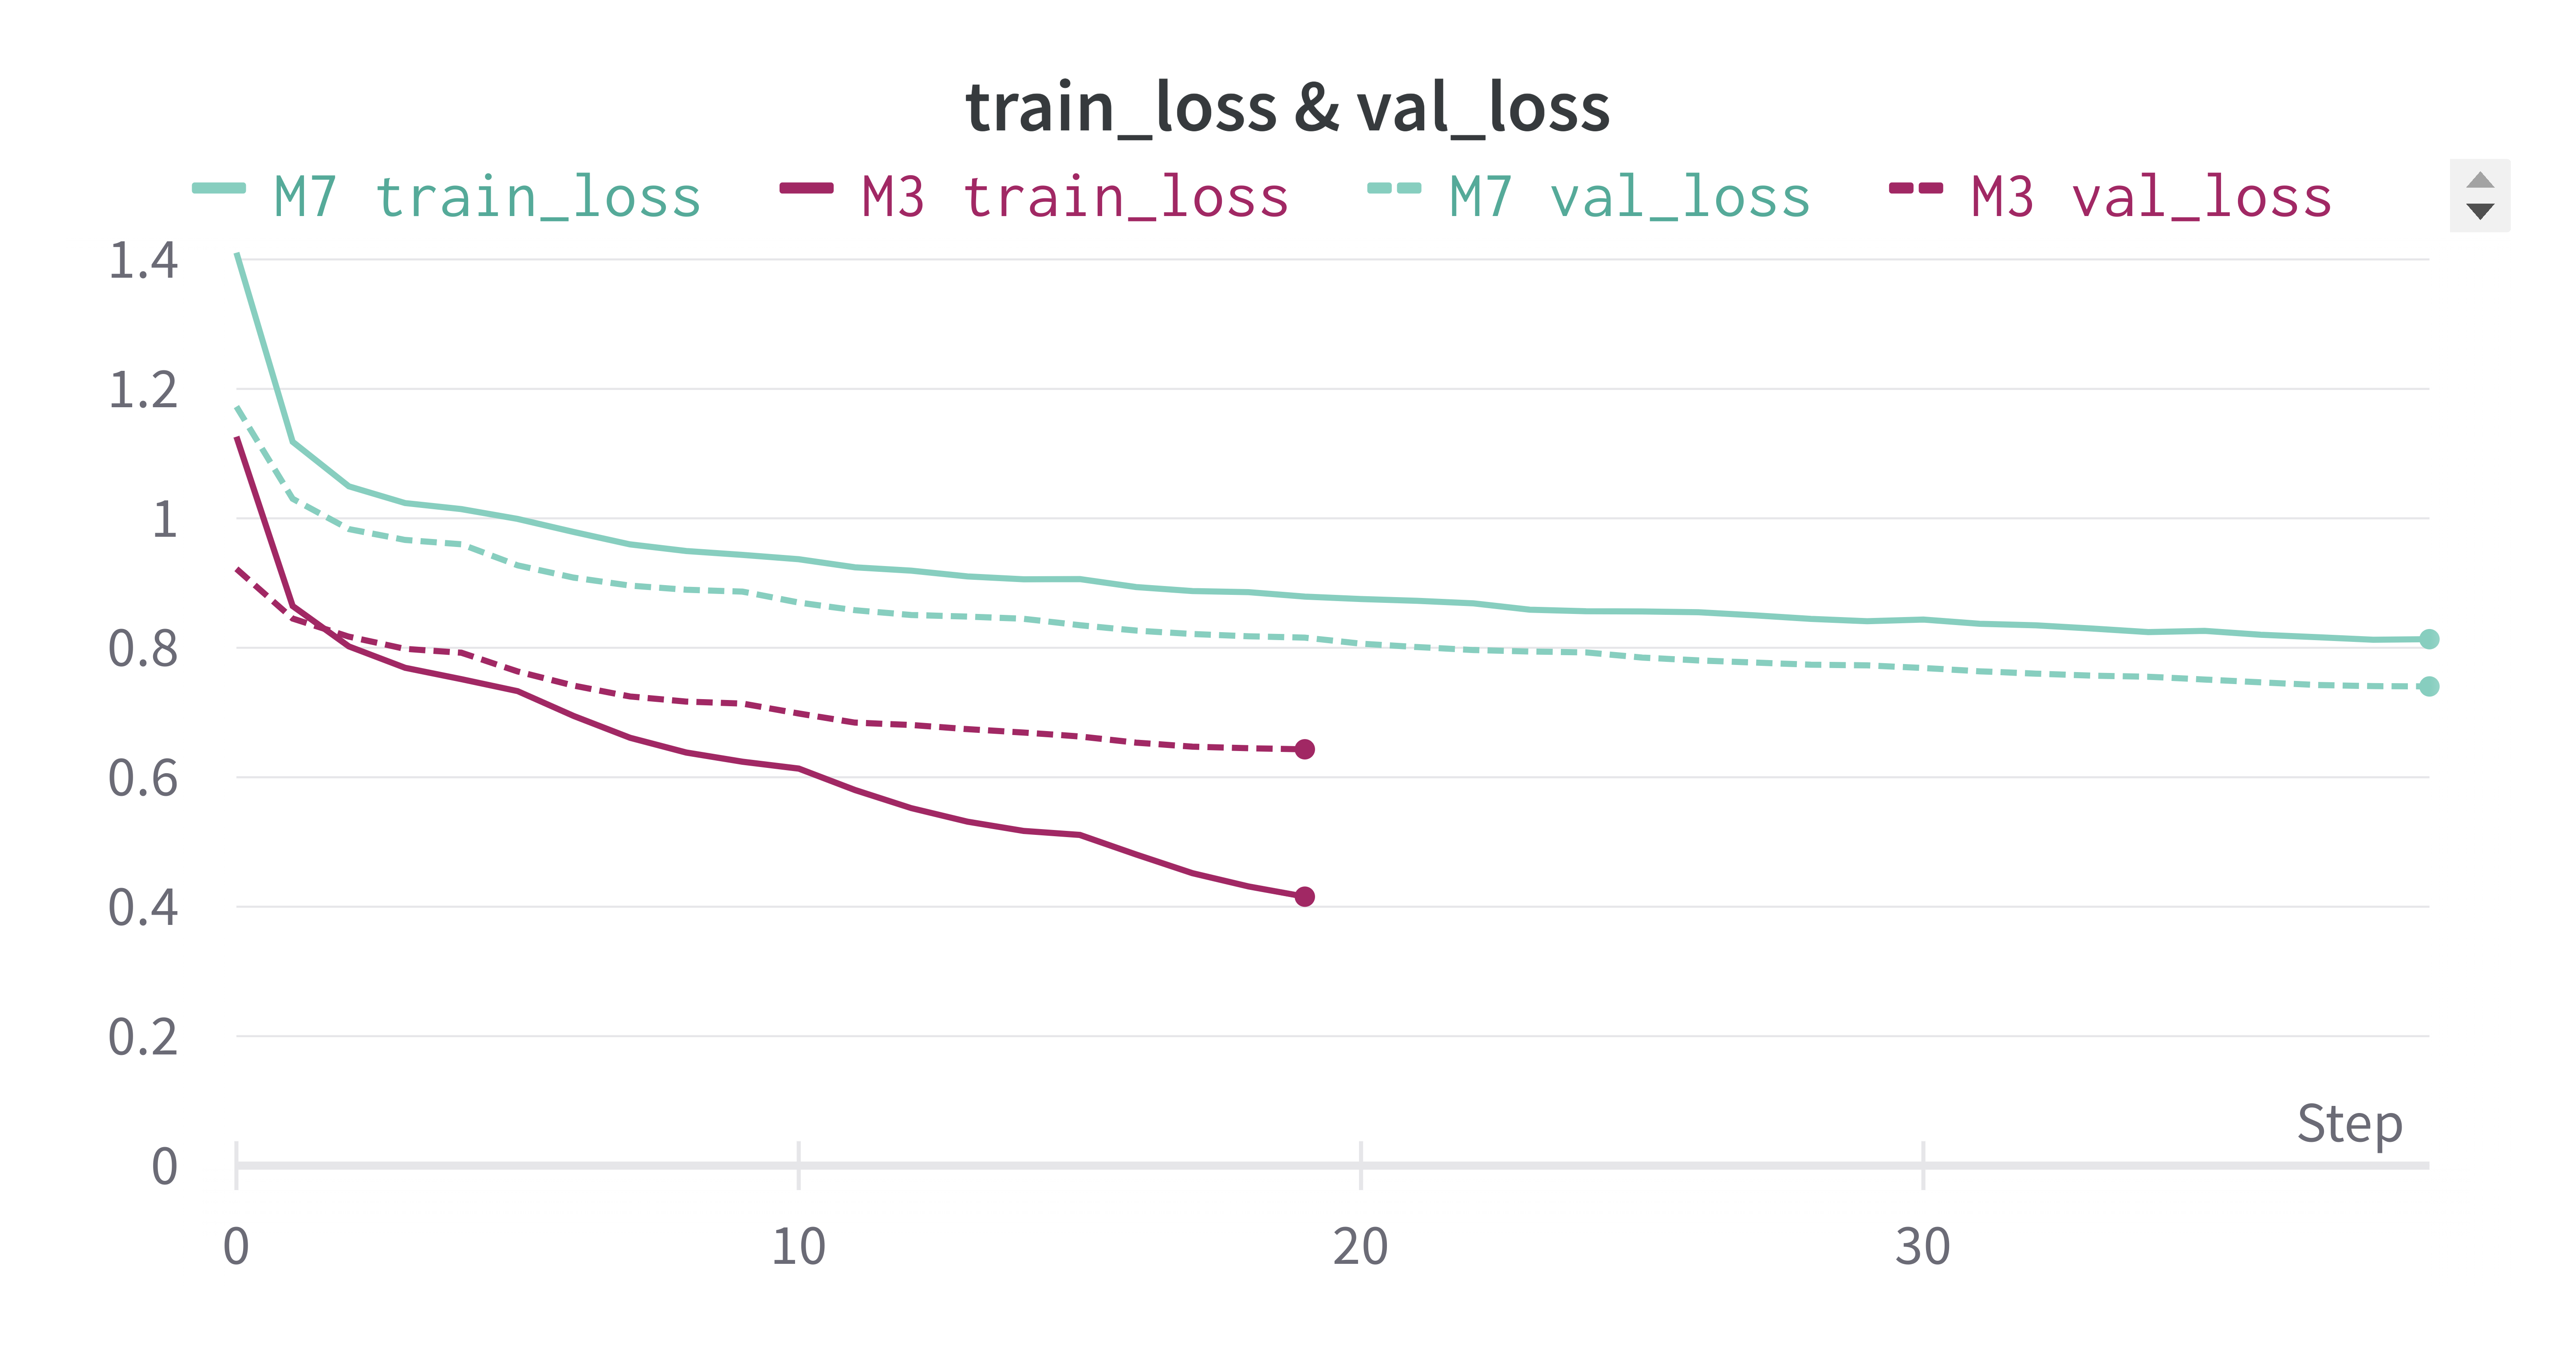
\includegraphics[width=\textwidth]{imatges/results/LossM3M7.png}
\caption[M3 vs. M7, Loss Train and Validation Curves]{\textit{M3 vs. M7, Loss Train and Validation Curves. Illustration by Author}}
{\label{fig:lossm0m4}}
\end{figure}

\newpage

\begin{figure}[H]
\centering
    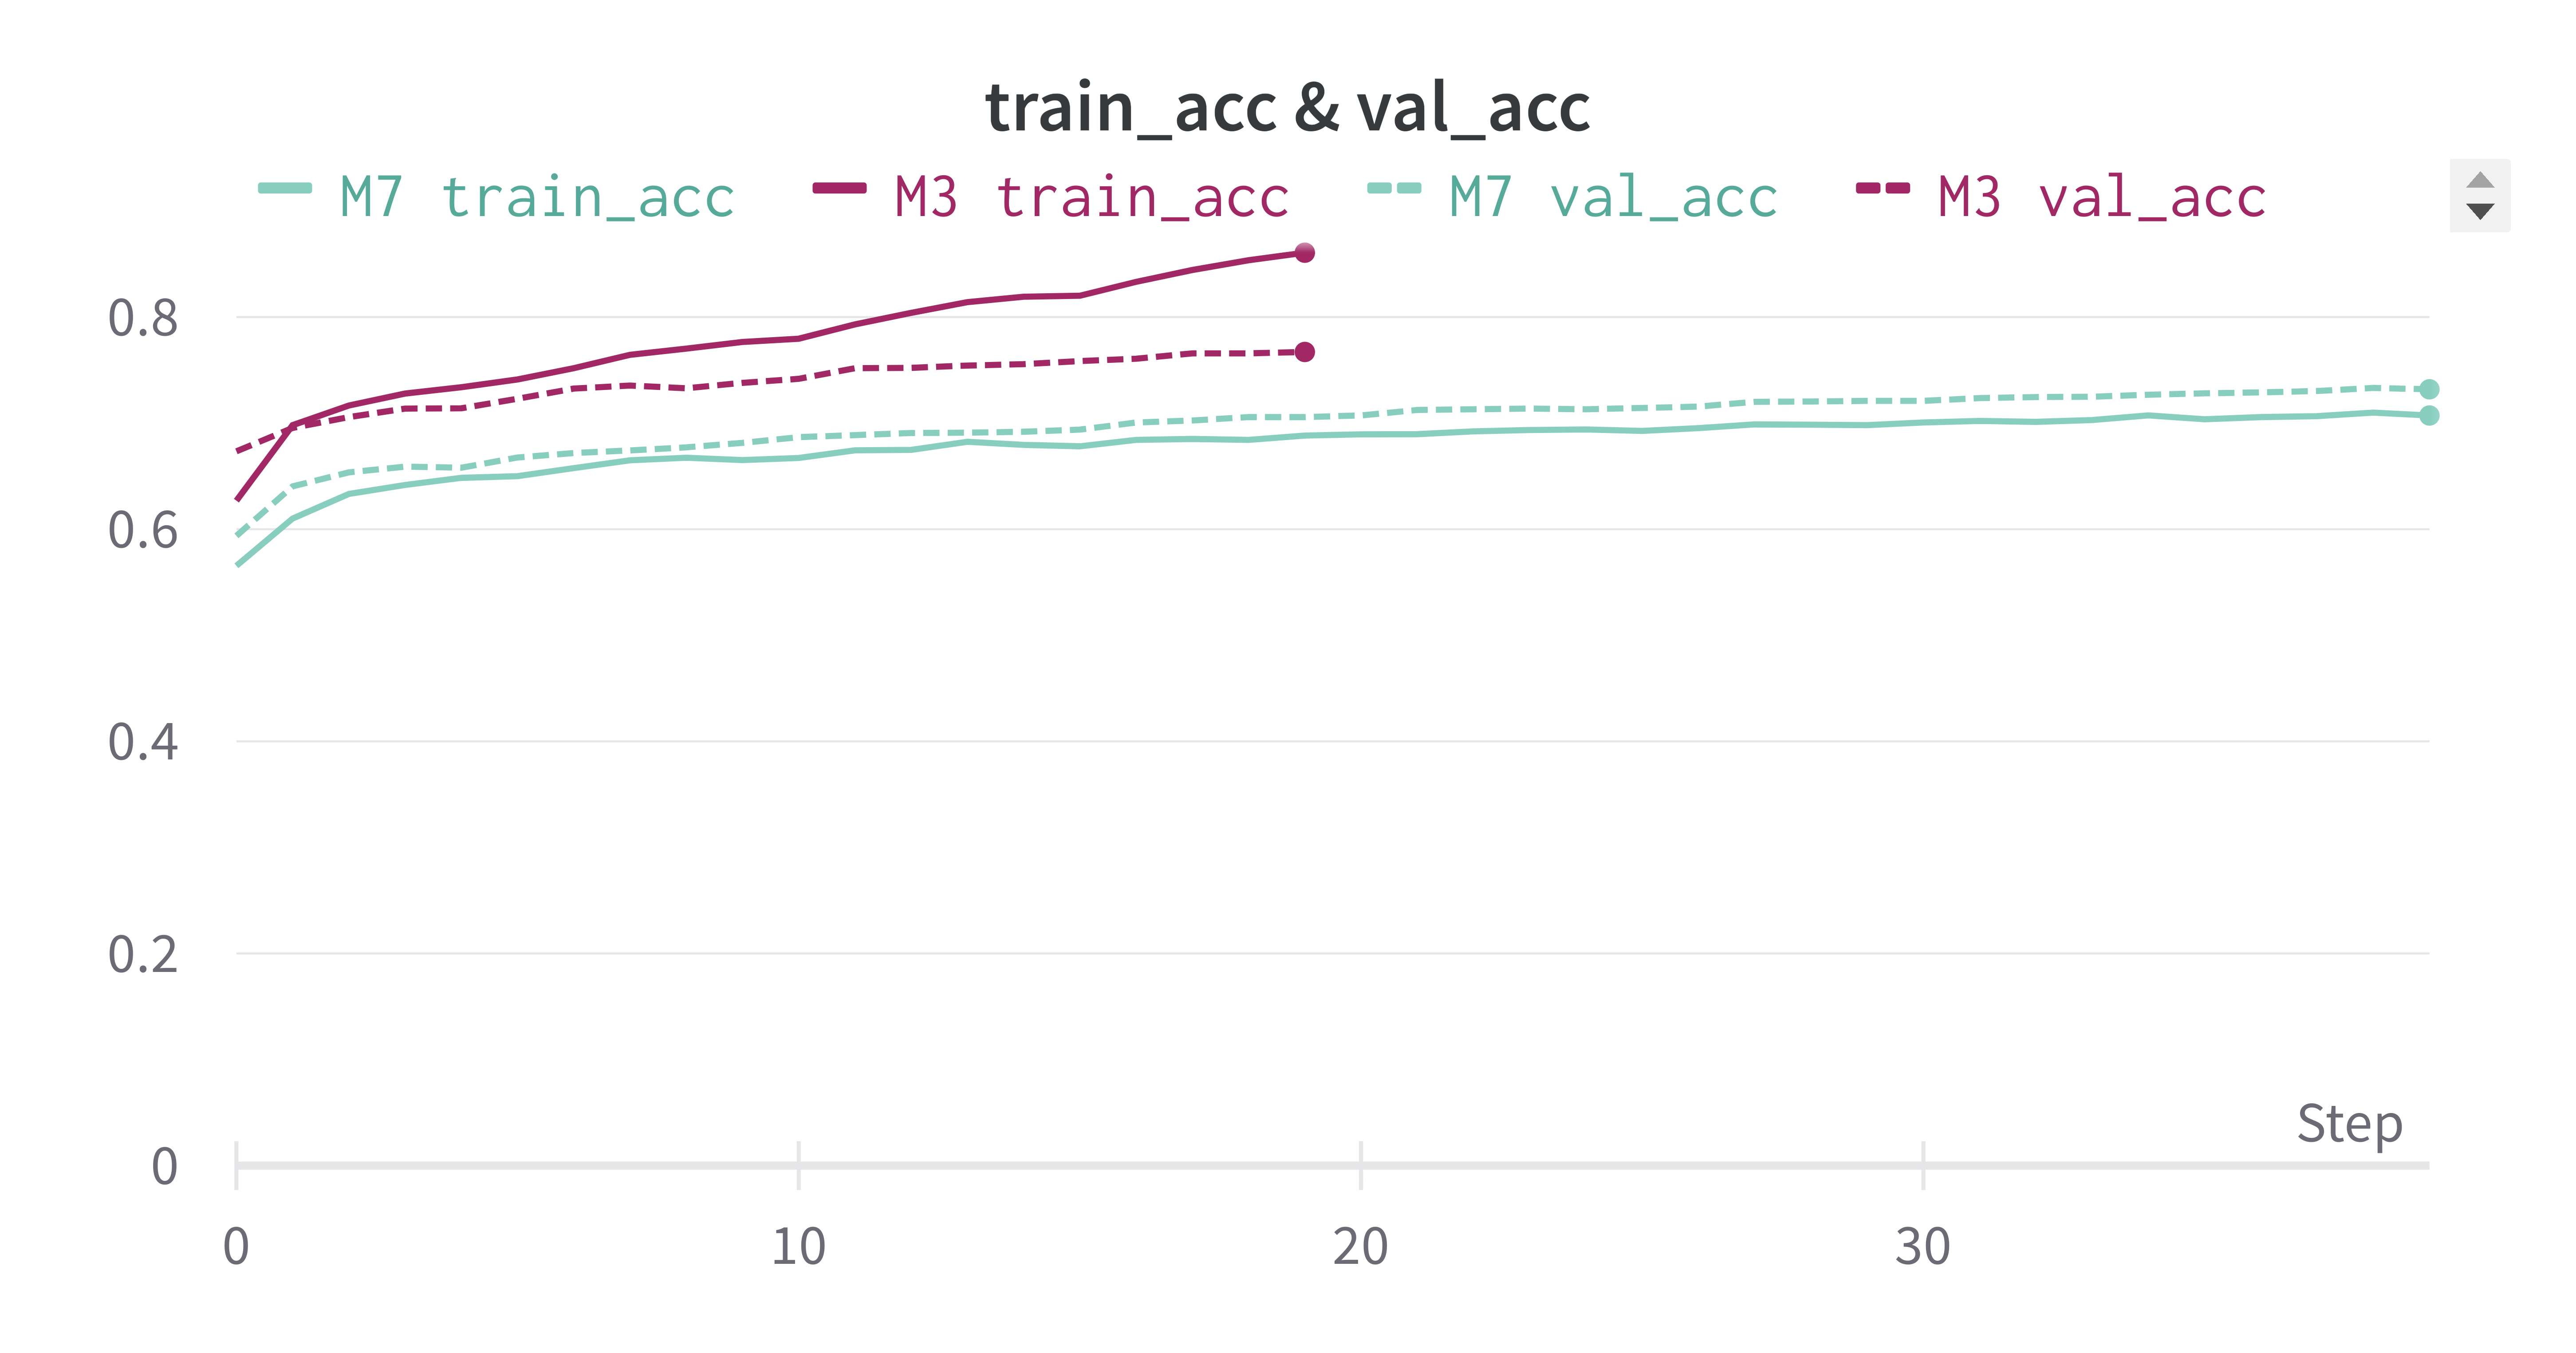
\includegraphics[width=\textwidth]{imatges/results/AccM3M7.png}
\caption[M3 vs. M7, Acc Train and Validation Curves]{\textit{M3 vs. M7, Acc Train and Validation Curves. Illustration by Author}}
{\label{fig:accm0m4}}
\end{figure}


\section{Testing}
